\documentclass[12pt,letterpaper]{report}
\usepackage[utf8]{inputenc}
\usepackage[spanish,mexico]{babel}
\usepackage{mathptmx}
\usepackage[top=2.5cm,bottom=2.5cm,left=3cm,right=2.5cm]{geometry}
\usepackage{amsmath,graphicx,booktabs,longtable,tabularx,array,multirow,ragged2e}
\usepackage[svgnames]{xcolor}
\definecolor{PasoColor}{HTML}{2E7D32}
\definecolor{FalloColor}{HTML}{C62828}
\definecolor{PendienteColor}{HTML}{757575}
\definecolor{AzulLink}{HTML}{1565C0}
\usepackage[colorlinks=true,linkcolor=AzulLink,citecolor=AzulLink,urlcolor=AzulLink]{hyperref}
\AtBeginDocument{\hypersetup{pdftitle={SQAP, ISO/IEC 25000 y JMeter -- SpeechNotes},pdfauthor={Consultora de Calidad Externa}}}
\usepackage{fancyhdr}
\pagestyle{fancy}
\fancyhf{}
\fancyhead[LE]{\textit{SpeechNotes -- SQAP}}
\fancyhead[RO]{\textit{Sección \thesection\ -- \leftmark}}
\fancyfoot[C]{\thepage}
\setlength{\headheight}{30pt}
\setlength{\emergencystretch}{3em}
\renewcommand{\headrulewidth}{0.4pt}
\usepackage{titlesec}
\titleformat{\chapter}{\normalfont\huge\bfseries}{\thechapter}{20pt}{\huge}
\titleformat{\section}{\normalfont\Large\bfseries}{\thesection}{16pt}{\Large}
\titleformat{\subsection}{\normalfont\large\bfseries}{\thesubsection}{12pt}{\large}
\usepackage{enumitem}
\setlist{nosep,leftmargin=*}
\usepackage{caption,float,pdflscape}
\begin{document}
\begin{titlepage}
\definecolor{EspeColor}{HTML}{1A5276}
\definecolor{AccentColor}{HTML}{2980B9}
\definecolor{SoftBg}{HTML}{F4F6F7}

\begin{center}
    \vspace*{0.5cm}
    
    % ── Logo Institucional ──
    
\includegraphics[width=0.45\textwidth]{imgs/espe-logo.png}\\[0.8cm]
    
    % ── Encabezado ──
    {\LARGE \textcolor{EspeColor}{\bfseries UNIVERSIDAD DE LAS FUERZAS ARMADAS ESPE}}\\[0.3cm]
    {\Large \textcolor{AccentColor}{\bfseries DEPARTAMENTO DE CIENCIAS DE LA COMPUTACIÓN}}\\[0.2cm]
    {\large \textbf{Aseguramiento de la Calidad de Software}}
    
    \vspace{1cm}
    
    % ── Separador Superior ──
    \textcolor{EspeColor}{\rule{\textwidth}{2.5pt}}
    \vspace{0.8cm}
    
    % ── Título del Documento ──
    {\Huge \textcolor{EspeColor}{\bfseries Plan de Aseguramiento de la Calidad}}\\[0.4cm]
    {\Huge \textcolor{EspeColor}{\bfseries de Software (SQAP)}}
    
    \vspace{0.8cm}
    % ── Separador Inferior ──
    \textcolor{EspeColor}{\rule{\textwidth}{2.5pt}}
    
    \vspace{1.2cm}
    
    % ── Detalles del Proyecto (Caja de color) ──
    \fcolorbox{EspeColor}{SoftBg}{
        \begin{minipage}{0.85\textwidth}
            \centering
            \vspace{0.4cm}
            {\Large \textcolor{AccentColor}{\bfseries PROYECTO}}\\[0.3cm]
            {\LARGE \bfseries SpeechNotes}\\[0.2cm]
            {\large Sistema de Transcripción Inteligente con IA}
            \vspace{0.4cm}
        \end{minipage}
    }
    
    \vspace{1.5cm}
    
    % ── Integrantes ──
    \fcolorbox{EspeColor}{white}{
        \begin{minipage}{0.75\textwidth}
            \centering
            \vspace{0.4cm}
            {\Large \textcolor{EspeColor}{\bfseries INTEGRANTES}}\\[0.5cm]
            \begin{tabular}{>{\large}l @{\hspace{2cm}} >{\large}l}
                $\bullet$ \textbf{Mesías Mariscal} & $\bullet$ \textbf{Julio Viche} \\[0.4cm]
                $\bullet$ \textbf{Denise Rea}      & $\bullet$ \textbf{Gabriel Murillo} \\
            \end{tabular}
            \vspace{0.4cm}
        \end{minipage}
    }
    
    \vfill
    
    % ── Footer de Portada ──
    \textcolor{AccentColor}{\rule{0.6\textwidth}{1pt}}\\[0.3cm]
    {\large \textcolor{EspeColor}{\textbf{Fecha de Entrega:}} Julio 2026}\\[0.1cm]
    {\small \textcolor{EspeColor}{\textit{Documento de Evaluación de Calidad SQA --- Versión 1.0}}}\\[0.1cm]
    {\small \textcolor{EspeColor}{\textit{Estándar de Referencia: IEEE Std 730-1998 / IEEE Std 730.1-1995}}}

\end{center}
\end{titlepage}

% ── Tabla de Revisiones ──
\chapter*{Registro de Revisiones}
\addcontentsline{toc}{chapter}{Registro de Revisiones}

\begin{longtable}{cccc}
\toprule
\textbf{Versión} & \textbf{Fecha} & \textbf{Descripción} & \textbf{Autor}\\
\midrule
1.0 & Julio 2026 & Versión inicial del SQAP & Consultora de Calidad\\
\bottomrule
\end{longtable}

\newpage

% ── Tabla de Contenidos ──
\tableofcontents
\newpage

\chapter{Propósito}
\label{sec:proposito}

El presente Plan de Aseguramiento de la Calidad de Software (SQAP) establece la organización, las tareas, las responsabilidades y los lineamientos para las actividades de aseguramiento de la calidad del proyecto \textbf{SpeechNotes}. Este documento sigue los lineamientos de los estándares IEEE 730-1998 e IEEE 730.1-1995, adaptados al contexto académico del proyecto final de SQA.

\section{Alcance}
\label{sec:alcance}

Este plan cubre las actividades de SQA realizadas durante el sprint de calidad comprendido entre el 18 y el 21 de julio de 2026.

\subsection{Módulos incluidos}
\label{subsec:modulos-incluidos}

A continuación se detallan los módulos y requisitos funcionales evaluados, junto con la justificación de su inclusión:

\begin{itemize}
    \item \textbf{RF-01 --- Auth (Autenticación y Sesiones):} Inicio de sesión con usuario demo y manejo de credenciales inválidas. \textit{Justificación:} Componente crítico de seguridad y control de acceso que actúa como puerta de entrada a la aplicación.
    \item \textbf{RF-02 --- Audio / Frontend (Captura de Dispositivo):} Prueba de micrófono con y sin dispositivo físico conectado. \textit{Justificación:} Verifica la capacidad de la interfaz web para interactuar con la Web Audio API del navegador y manejar excepciones de hardware.
    \item \textbf{RF-03 --- Audio / Backend (Procesamiento VAD):} Inicio y detención de grabación con detección de actividad de voz (Voice Activity Detection). \textit{Justificación:} El motor VAD determina los segmentos de voz válidos, reduciendo datos nulos antes de enviarlos a transcripción.
    \item \textbf{RF-04 --- Realtime ASR (Transcripción en Vivo):} Streaming WebSocket de fragmentos de audio y transcripción continua. \textit{Justificación:} Flujo principal (Core Business Flow) donde la latencia y sincronización determinan la experiencia del usuario.
    \item \textbf{RF-05 --- Upload / Backend (Ingesta de Audio):} Carga de archivos de audio (WAV, MP3, 0-bytes) para transcripción asíncrona. \textit{Justificación:} Permite procesar grabaciones preexistentes y validar el manejo de formatos e insumos corruptos o vacíos.
    \item \textbf{RF-06 --- Transcripciones (Persistencia y Consulta):} Recuperación de transcripciones guardadas en MongoDB/SQLite. \textit{Justificación:} Asegura la integridad del almacenamiento persistente de las notas generadas.
    \item \textbf{RF-07 --- Editor (Edición de Contenido):} Modificación de texto transcrito y guardado de cambios. \textit{Justificación:} Permite la corrección manual del texto generado por el modelo de IA antes de su formateo final.
    \item \textbf{RF-08 --- Búsqueda (Búsqueda Textual):} Filtrado de transcripciones por palabras clave. \textit{Justificación:} Garantiza la correcta localización de información en historiales extensos.
    \item \textbf{RF-09 --- IA / Formatter (Estructuración con LLM):} Formateo automatizado de notas mediante el pipeline de NVIDIA NIM. \textit{Justificación:} Transforma transcripciones crudas en notas estructuradas (puntos clave, resúmenes, minutas).
    \item \textbf{RF-10 --- Chat / RAG (Asistente Contextual):} Interacción conversacional sobre el contenido de la transcripción. \textit{Justificación:} Funcionalidad avanzada de búsqueda semántica y recuperación aumentada por generación sobre los documentos del usuario.
\end{itemize}

\subsection{Módulos excluidos}
\label{subsec:modulos-excluidos}

Se delimitan los siguientes componentes y pruebas fuera del alcance del presente plan:

\begin{itemize}
    \item \textbf{Pruebas de carga y estrés prolongadas (> 2 horas):} Excluidas debido al consumo intensivo y límites de cuotas operativas de las APIs de GPU en NVIDIA NIM Cloud, concentrando el análisis de rendimiento en pruebas de integración y carga puntual.
    \item \textbf{Automatización E2E al 100\% de cobertura:} Excluida por las limitaciones de tiempo del sprint de SQA. Se priorizó una estrategia híbrida con automatización focalizada (backend con \texttt{pytest} y escenarios críticos con \texttt{Cypress}) complementada con ejecución manual exhaustiva.
    \item \textbf{Refactorización y corrección directa de código base:} Excluida por delimitación de roles. El equipo de SQA identifica, documenta y reporta defectos en Jira, siendo responsabilidad del equipo de desarrollo la implementación de parches.
    \item \textbf{Configuración inicial e infraestructura de SonarCloud:} Se toma la instancia y reglas de calidad previamente desplegadas como línea base operacional para el análisis estático.
\end{itemize}

\section{Identificación del Sistema}
\label{sec:identificacion}

\begin{itemize}
    \item \textbf{Nombre:} SpeechNotes
    \item \textbf{Versión:} 1.0
    \item \textbf{Repositorio:} \url{https://github.com/gamurigm/SpeechNotes}
    \item \textbf{Rama SQA:} \texttt{planning-SQA}
\end{itemize}

\section{Resumen del Sistema}
\label{sec:resumen}

SpeechNotes es un sistema de transcripción inteligente que convierte audio en notas estructuradas mediante un pipeline de cinco modelos especializados de NVIDIA NIM. La arquitectura sigue un patrón de tres capas:

\begin{itemize}
    \item \textbf{Frontend:} Next.js 16 con HeroUI, Socket.IO Client y soporte para aplicaciones de escritorio (Tauri/Electron).
    \item \textbf{Backend:} FastAPI con Socket.IO, servicios modulares de audio (ASR, BNR, VAD) y agentes de IA para formateo y chat contextual.
    \item \textbf{Datos y Modelos:} MongoDB (primario), SQLite/Prisma (auth), ChromaDB (búsqueda vectorial) y NVIDIA NIM (modelos de IA).
\end{itemize}

\section{Resumen del Documento}
\label{sec:resumen-doc}

Este SQAP se estructura en 15 secciones y 5 apéndices, mapeando los requisitos del estándar académico (Secciones A, B, C, D) de la siguiente manera:

\begin{itemize}
    \item \textbf{Sección A (Plan SQAP):} Capítulos 1 al 5 y 14.
    \item \textbf{Sección B (Ejecución y Evidencias):} Capítulos 6 y 7, Apéndices A al D.
    \item \textbf{Sección C (Informe de Cierre):} Apéndice E.
    \item \textbf{Sección D (Conclusiones):} Capítulo 15.
\end{itemize}

\section{Relación con Otros Planes}
\label{sec:relacion}

Este SQAP se complementa con el Plan de Desarrollo de Software (SDP) y el Plan de Gestión de Configuración (SCMP) del proyecto SpeechNotes. Las actividades de SQA definidas aquí son consistentes con dichos planes.

\section{Documentos Oficiales de Referencia}
\label{sec:referencias}

Los documentos normativos oficiales utilizados como referencia para este SQAP son:

\begin{enumerate}
    \item IEEE Std 730-1998 --- IEEE Standard for Software Quality Assurance Plans.
    \item IEEE Std 730.1-1995 --- IEEE Guide for Software Quality Assurance Planning.
    \item IEEE/EIA Std 12207 --- Standard for Information Technology -- Software Life Cycle Processes.
\end{enumerate}

\chapter{Gestión}
\label{sec:gestion}

Este capítulo describe los elementos organizacionales que influyen en la calidad del software de SpeechNotes.

\section{Organización}
\label{sec:organizacion}

El equipo SQA está compuesto por 4 personas con roles definidos, manteniendo independencia funcional respecto al equipo de desarrollo. La estructura organizacional se muestra en la Figura~\ref{fig:organigrama}.

\begin{figure}[H]
\centering
\fbox{\parbox{0.8\textwidth}{\centering
\textbf{Project Manager}\\
$\downarrow$\\[-0.2cm]
\textbf{Consultora de Calidad (Externa)}\\
$\swarrow$ \quad $\downarrow$ \quad $\searrow$\\[-0.2cm]
\begin{tabular}{ccc}
\textbf{Pers. A} & \textbf{Pers. B} & \textbf{Pers. C}\\
QA Lead & QA Backend & QA Frontend\\
& + CI/CD & \\
\end{tabular}\\
$\downarrow$\\[-0.2cm]
\textbf{Pers. D}\\
QA Manual
}}
\caption{Organigrama del equipo SQA}
\label{fig:organigrama}
\end{figure}

\section{Responsabilidades}
\label{sec:responsabilidades}

La tabla~\ref{tab:responsabilidades} detalla las responsabilidades asignadas a cada miembro del equipo.

\begin{longtable}{cp{5cm}p{7cm}}
\caption{Matriz de responsabilidades SQA}
\label{tab:responsabilidades}\\
\toprule
\textbf{Rol} & \textbf{Responsable} & \textbf{Tareas Clave}\\
\midrule
\endfirsthead
\toprule
\textbf{Rol} & \textbf{Responsable} & \textbf{Tareas Clave}\\
\midrule
\endhead
\bottomrule
\endfoot

QA Lead & Persona A & Configuración de Jira, redacción del SQAP (Sección A), informe de cierre (Sección C), conclusiones (Sección D), ensamblaje del PDF final.\\

QA Backend & Persona B & Pipeline SonarCloud + GitHub Actions, pruebas automatizadas pytest, refactorización de code smells, reporte de análisis estático antes/después.\\

QA Frontend & Persona C & Configuración de Cypress/Jest, automatización de flujos clave (grabación, transcripción), corrección de bugs frontend reportados.\\

QA Manual & Persona D & Diseño de matriz de rastreabilidad, casos de prueba manuales (14 CP), ejecución manual, reporte de bugs en Jira, re-testing, video demo.\\

\end{longtable}

\section{Recursos}
\label{sec:recursos}

\subsection{Equipo y ambiente de prueba}
\label{subsec:ambiente}

\begin{itemize}
    \item \textbf{Sistema Operativo:} Windows 11.
    \item \textbf{Navegador:} Google Chrome / Chromium.
    \item \textbf{Frontend:} \url{http://localhost:3006}
    \item \textbf{Backend:} \url{http://localhost:9443}
    \item \textbf{Base de datos:} SQLite (dev.db) + MongoDB (Docker).
    \item \textbf{Repositorio:} GitHub, rama \texttt{planning-SQA}.
\end{itemize}

\subsection{Herramientas}
\label{subsec:herramientas}

\begin{itemize}
    \item \textbf{Gestión de incidencias:} Jira Software (Cloud).
    \item \textbf{Análisis estático:} SonarCloud.
    \item \textbf{CI/CD:} GitHub Actions.
    \item \textbf{Pruebas backend:} pytest.
    \item \textbf{Pruebas frontend:} Cypress + Jest.
    \item \textbf{Consola API:} curl / Postman.
    \item \textbf{Evidencias:} Capturas de pantalla, logs de backend, consola del navegador.
\end{itemize}

\chapter{Tareas SQA}
\label{sec:tareas}

Este capítulo describe las tareas de aseguramiento de la calidad ejecutadas durante el sprint.

\section{Revisión de Productos de Software}
\label{sec:revision-productos}

SQA revisó los siguientes productos de software:

\begin{itemize}
    \item Código fuente del backend (Python/FastAPI) y frontend (TypeScript/Next.js).
    \item Documentación técnica (README, guías de despliegue, documentación de arquitectura).
    \item Transcripciones generadas (formato Markdown con metadatos YAML).
    \item Configuración de infraestructura (Docker, GitHub Actions, SonarCloud).
\end{itemize}

\section{Evaluación de Herramientas}
\label{sec:evaluacion-herramientas}

Se evaluaron las siguientes herramientas utilizadas en el proyecto:

\begin{longtable}{lcp{7cm}}
\caption{Evaluación de herramientas SQA}
\label{tab:herramientas-evaluadas}\\
\toprule
\textbf{Herramienta} & \textbf{Propósito} & \textbf{Resultado}\\
\midrule
\endfirsthead
\toprule
\textbf{Herramienta} & \textbf{Propósito} & \textbf{Resultado}\\
\midrule
\endhead
\bottomrule
\endfoot

Jira Cloud & Gestión de incidencias y bugs & Configurado con flujo To Do $\rightarrow$ In Progress $\rightarrow$ In Testing $\rightarrow$ Done.\\

SonarCloud & Análisis estático de código & Pipeline GitHub Actions configurado. Reporte inicial generado.\\

pytest & Pruebas unitarias e integración backend & Suite configurada en \texttt{backend/tests/}.\\

Cypress & Pruebas E2E frontend & Suite configurada en \texttt{web/tests/e2e/}.\\

Jest & Pruebas unitarias frontend & Suite configurada en \texttt{web/tests/unit/}.\\

\end{longtable}

La Figura~\ref{fig:tablero-jira-sqa} evidencia el seguimiento operativo de las actividades del sprint en Jira, incluyendo responsables, fechas objetivo y estados de ejecución.

\begin{figure}[H]
\centering
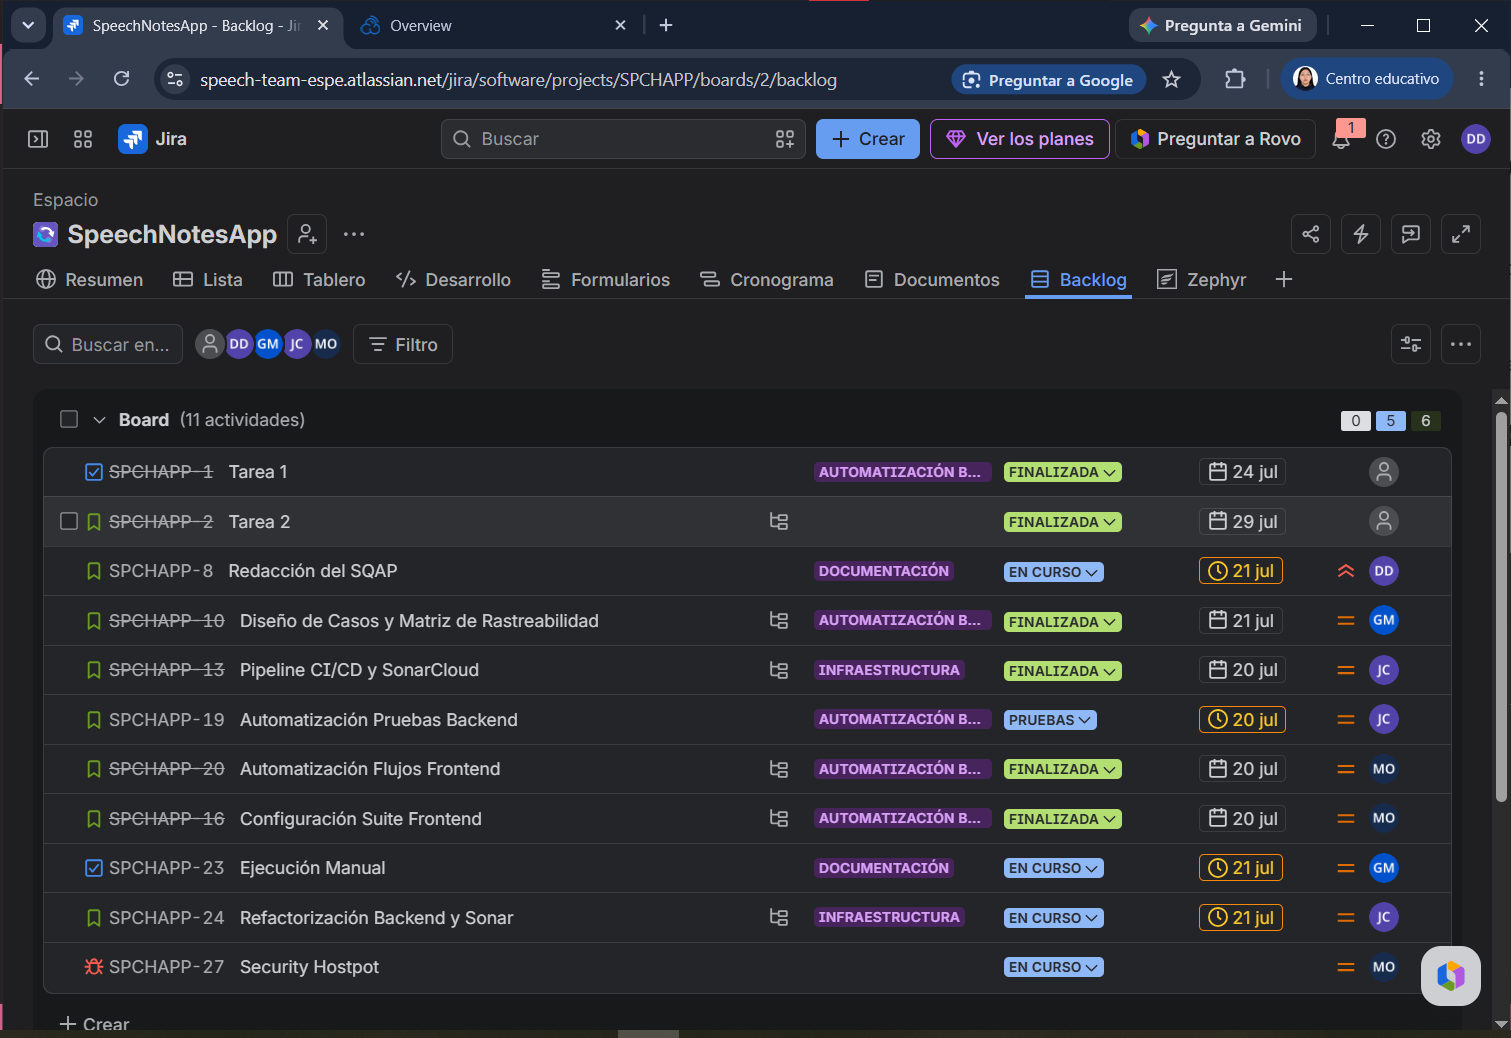
\includegraphics[width=\textwidth]{../../informe/images/tablero-kanban.png}
\caption{Tablero Jira utilizado para el seguimiento de actividades SQA}
\label{fig:tablero-jira-sqa}
\end{figure}

\section{Verificación de Procesos}
\label{sec:verificacion-procesos}

SQA verificó los siguientes procesos mediante auditorías basadas en checklist:

\begin{enumerate}
    \item \textbf{Planificación y seguimiento:} Cumplimiento del sprint planificado (18-21 Julio).
    \item \textbf{Gestión de requisitos:} Trazabilidad entre requisitos funcionales y casos de prueba.
    \item \textbf{Diseño e implementación:} Calidad del código y aplicación de patrones de diseño.
    \item \textbf{Pruebas:} Cobertura de casos de prueba y reporte de defectos.
\end{enumerate}

\section{Auditorías de Configuración}
\label{sec:auditorias-configuracion}

Se verificó el control de configuración mediante:

\begin{itemize}
    \item Repositorio Git con rama dedicada \texttt{planning-SQA}.
    \item Flujo de trabajo basado en feature branches + pull requests.
    \item Pipeline de CI/CD en GitHub Actions para pruebas y análisis estático.
\end{itemize}

\section{Cronograma}
\label{sec:cronograma}

El sprint de calidad se ejecutó en 4 días según el siguiente cronograma:

\begin{longtable}{lcp{6cm}}
\caption{Cronograma del sprint SQA}
\label{tab:cronograma}\\
\toprule
\textbf{Día} & \textbf{Fecha} & \textbf{Actividades}\\
\midrule
\endfirsthead
\toprule
\textbf{Día} & \textbf{Fecha} & \textbf{Actividades}\\
\midrule
\endhead
\bottomrule
\endfoot

1 & 18 Jul & Planificación, configuración de Jira, análisis estático inicial (SonarCloud), diseño de casos de prueba y matriz de rastreabilidad.\\

2 & 19 Jul & Ejecución manual de pruebas, reporte de bugs, pruebas automatizadas backend (pytest) y frontend (Cypress/Jest).\\

3 & 20 Jul & Re-testing de bugs corregidos, análisis estático final (SonarCloud después), extracción de evidencias.\\

4 & 21 Jul & Consolidación del PDF final, grabación del video demo, cierre del informe.\\

\end{longtable}

\chapter{Estándares, Prácticas, Convenciones y Métricas}
\label{sec:estandares}

\section{Estándares de Código}
\label{sec:estandares-codigo}

El proyecto SpeechNotes sigue los siguientes estándares y convenciones:

\begin{longtable}{lp{4cm}p{6cm}}
\caption{Estándares de código aplicados}
\label{tab:estandares-codigo}\\
\toprule
\textbf{Lenguaje} & \textbf{Estándar} & \textbf{Herramienta de verificación}\\
\midrule
\endfirsthead
\toprule
\textbf{Lenguaje} & \textbf{Estándar} & \textbf{Herramienta de verificación}\\
\midrule
\endhead
\bottomrule
\endfoot

Python & PEP 8 & Ruff / SonarCloud\\

TypeScript & ESLint + Prettier & SonarCloud\\

Arquitectura & Patrones GoF (Singleton, Factory, Adapter, Facade, Strategy, State, Observer) & Revisiones de código\\

Base de datos & Prisma ORM + MongoDB & Linting de esquema\\

\end{longtable}

\section{Métricas SQA}
\label{sec:metricas}

Las siguientes métricas fueron recolectadas para evaluar la calidad del producto y del proceso de pruebas:

\subsection{Porcentaje de casos pasados vs.\ fallados}
\label{subsec:porcentaje-casos}

\[
\%\text{Pasados} = \frac{\text{Casos pasados}}{\text{Total casos}} \times 100
\]

\subsection{Densidad de defectos}
\label{subsec:densidad-defectos}

\[
\text{Densidad de defectos} = \frac{\text{Número de defectos encontrados}}{\text{Número de casos de prueba ejecutados}}
\]

\subsection{Cobertura de requisitos}
\label{subsec:cobertura-rf}

\[
\%\text{Cobertura RF} = \frac{\text{Requisitos con al menos un caso asociado}}{\text{Total requisitos funcionales}} \times 100
\]

\subsection{Periodicidad de reporte}
\label{subsec:periodicidad}

Las métricas fueron reportadas al finalizar el sprint de calidad (21 de julio de 2026), consolidadas en el Apéndice~E (Informe de Cierre).

\chapter{Estrategia y Tipos de Prueba}
\label{sec:pruebas}

\section{Tipos de Prueba Seleccionados}
\label{sec:tipos-prueba}

La estrategia de pruebas sigue una pirámide de pruebas adaptada a arquitecturas con componentes de Inteligencia Artificial y streaming en tiempo real:

\begin{enumerate}[label=\alph*)]
    \item \textbf{Pruebas Unitarias (Backend y Frontend):} Evalúan la lógica interna de funciones aisladas sin dependencias de red o base de datos. Se utiliza \texttt{pytest} en el backend para validar algoritmos de VAD, utilidades de formateo y servicios de tokenización; y \texttt{Jest} en el frontend para probar componentes aislados como \texttt{RecordingPanel} y \texttt{LiveTranscription}.
    \item \textbf{Pruebas de Integración (Backend):} Verifican la interacción entre módulos del sistema (p.~ej., FastApi con SQLite/Prisma, motor de Socket.IO con el pipeline de audio y clientes HTTP con NVIDIA NIM). Se utiliza \texttt{pytest} con \texttt{httpx} para simular peticiones asíncronas a los endpoints REST.
    \item \textbf{Pruebas Funcionales / Sistema (Manuales y Exploratorias):} Validan de extremo a extremo los flujos de usuario sobre la interfaz web completa y APIs REST. Se ejecutaron 17 casos de prueba estructurados (Apéndice~\ref{apendice:b}) cubriendo flujos exitosos (\textit{Happy Path}), condiciones de error y escenarios de seguridad.
    \item \textbf{Pruebas de Análisis Estático (SAST):} Inspección continua del código fuente mediante \texttt{SonarCloud} para identificar vulnerabilidades de seguridad, violaciones de estándares de codificación, duplidado de código y \textit{code smells}.
    \item \textbf{Pruebas E2E / Interfaz (Automatizadas):} Pruebas en navegador con \texttt{Cypress} para simular las interacciones completas del usuario en la interfaz Next.js, incluyendo flujos de autenticación, carga de archivos y manipulación del editor.
\end{enumerate}

\begin{longtable}{llp{5cm}}
\caption{Resumen de tipos de prueba ejecutados}
\label{tab:tipos-prueba}\\
\toprule
\textbf{Tipo} & \textbf{Herramienta} & \textbf{Alcance}\\
\midrule
\endfirsthead
\toprule
\textbf{Tipo} & \textbf{Herramienta} & \textbf{Alcance}\\
\midrule
\endhead
\bottomrule
\endfoot

Unitarias (Backend) & pytest & Servicios individuales de audio, VAD, auth\\

Integración (Backend) & pytest + httpx & Endpoints REST: transcriptions, auth, health\\

Funcionales Manuales & Navegador + curl & 17 casos de prueba (Apéndice~B)\\

Estáticas & SonarCloud & Análisis de código, code smells, vulnerabilidades\\

E2E (Frontend) & Cypress & Flujo de grabación y transcripción\\

Unitarias (Frontend) & Jest & Componentes RecordingPanel, LiveTranscription\\

\end{longtable}

\section{Criterios de Aceptación y Rechazo}
\label{sec:criterios}

Para garantizar el rigor técnico del proceso SQA, se definen explícitamente los criterios de entrada y salida para el ciclo de pruebas:

\subsection{Criterios de entrada (Entry Criteria)}
\label{subsec:entry}

Una fase o suite de pruebas sólo podrá iniciarse cuando se cumplan las siguientes condiciones previas:

\begin{itemize}
    \item Frontend Next.js compilado y operativo en \url{http://localhost:3006}.
    \item Backend FastAPI iniciado y respondiendo health-checks en \url{http://localhost:9443}.
    \item Base de datos relacional/vectorial inicializada con esquemas vigentes (\texttt{web/dev.db}).
    \item Usuario de prueba estandarizado creado (\texttt{demo@speechnotes.app} / \texttt{demo123}).
    \item Dispositivo físico de captura de audio (micrófono) detectado e inicializado en la estación de pruebas.
    \item Claves de API activas y cuota disponible para los servicios externos de NVIDIA NIM Cloud.
    \item Matriz de rastreabilidad y casos de prueba revisados y aprobados por el líder SQA.
\end{itemize}

\subsection{Criterios de salida (Exit Criteria)}
\label{subsec:exit}

El ciclo de pruebas se considerará completado satisfactoriamente y el sistema estará listo para cierre cuando se alcancen las siguientes condiciones de aceptación:

\begin{itemize}
    \item El 100\% de los 17 casos de prueba diseñados hayan sido ejecutados y documentados.
    \item La tasa de éxito de casos de prueba quede documentada junto con los defectos asociados (alcanzado: 76.47\%; 4 fallas registradas).
    \item El 100\% de los defectos clasificados como severidad \texttt{Critical} haya sido corregido y verificado; los defectos \texttt{Major} abiertos deben quedar registrados con plan de remediación.
    \item Los defectos menores u opcionales pendientes estén formalmente registrados en Jira con su respectivo plan de remediación posterior.
    \item Se haya completado la ejecución del análisis estático en SonarCloud con revisión de \textit{Quality Gate}.
    \item El Informe de Cierre de SQA y la Matriz de Rastreabilidad estén consolidados y anexados al presente documento.
\end{itemize}

\section{Matriz de Pruebas vs.\ Requisitos}
\label{sec:matriz-pruebas}

La matriz de rastreabilidad completa se presenta en el Apéndice~\ref{apendice:a}. En resumen:

\begin{itemize}
    \item \textbf{10 requisitos funcionales} cubiertos al 100\%.
    \item \textbf{17 casos de prueba} distribuidos en 13 flujos funcionales y 4 condiciones negativas o de seguridad.
    \item \textbf{13 casos pasados} (76.47\%) y \textbf{4 casos fallados} (23.53\%); CP-09 se contabiliza como aprobado después de la re-prueba.
\end{itemize}

\chapter{Reporte y Resolución de No Cumplimientos}
\label{sec:reporte-resolucion}

\section{Proceso de Reporte de Defectos}
\label{sec:reporte-defectos}

Los defectos encontrados durante las pruebas se registraron en Jira siguiendo el siguiente flujo:

\begin{enumerate}
    \item \textbf{Reporte:} El tester crea un issue de tipo ``Bug'' en Jira.
    \item \textbf{Clasificación:} El QA Lead asigna severidad (\texttt{Critical}, \texttt{Major}, \texttt{Minor}) y prioridad.
    \item \textbf{Asignación:} El Project Manager asigna el bug al desarrollador responsable.
    \item \textbf{Corrección:} El desarrollador implementa la corrección y mueve el issue a ``In Testing''.
    \item \textbf{Verificación:} El tester re-ejecuta el caso de prueba y verifica la corrección.
    \item \textbf{Cierre:} Si el defecto está corregido, se cierra el issue. En caso contrario, se reabre.
\end{enumerate}

\section{Defectos Encontrados}
\label{sec:defectos-encontrados}

Los defectos encontrados se detallan en el Apéndice~C. A continuación se presenta un resumen:

\begin{longtable}{lccc}
\caption{Resumen de defectos}
\label{tab:resumen-defectos}\\
\toprule
\textbf{ID} & \textbf{Severidad} & \textbf{Estado} & \textbf{Caso Asociado}\\
\midrule
\endfirsthead
\toprule
\textbf{ID} & \textbf{Severidad} & \textbf{Estado} & \textbf{Caso Asociado}\\
\midrule
\endhead
\bottomrule
\endfoot

BUG-002 & Minor & Abierto & CP-03\\

BUG-003 & Critical & Cerrado & CP-10\\

BUG-004 & Major & Cerrado & CP-07\\

BUG-005 & Major & Abierto & CP-07\\

BUG-006 & Minor & Abierto & CP-01\\

BUG-007 & Minor & Cerrado & CP-03\\

BUG-008 & Minor & Abierto & CP-14\\

BUG-009 & Minor & Abierto & CP-05\\

\end{longtable}

\section{Resumen de Resultados}
\label{sec:resumen-resultados}

\begin{itemize}
    \item Total defectos: 8
    \item Defectos cerrados: 3 (BUG-003, BUG-004, BUG-007)
    \item Defectos abiertos: 5 (BUG-002, BUG-005, BUG-006, BUG-008, BUG-009)
    \item Tasa de cierre: 37.5\%
\end{itemize}

\chapter{Herramientas, Técnicas y Metodologías}
\label{sec:herramientas}

\section{Herramientas SQA}
\label{sec:herramientas-sqa}

La tabla~\ref{tab:herramientas-detalle} detalla las herramientas utilizadas en el proyecto.

\begin{longtable}{lp{3cm}p{5cm}p{3cm}}
\caption{Detalle de herramientas SQA}
\label{tab:herramientas-detalle}\\
\toprule
\textbf{Herramienta} & \textbf{Versión} & \textbf{Tipo} & \textbf{Propósito}\\
\midrule
\endfirsthead
\toprule
\textbf{Herramienta} & \textbf{Versión} & \textbf{Tipo} & \textbf{Propósito}\\
\midrule
\endhead
\bottomrule
\endfoot

Jira Software & Cloud & Gestión de proyectos & Seguimiento de tareas y defectos\\

SonarCloud & Cloud & Análisis estático & Medición de calidad de código\\

GitHub Actions & Cloud & CI/CD & Automatización de pruebas\\

pytest & 8.x & Automatización & Pruebas backend\\

Cypress & 14.x & Automatización & Pruebas E2E frontend\\

Jest & 29.x & Automatización & Pruebas unitarias frontend\\

Postman & Desktop & Manual & Pruebas de API\\

curl & CLI & Manual & Pruebas de API\\

\end{longtable}

\section{Justificación Técnica del Stack Elegido}
\label{sec:justificacion-stack}

La selección del conjunto de herramientas de SQA responde a criterios de compatibilidad con la arquitectura del sistema, eficiencia en ejecución asíncrona y adopción de estándares de la industria:

\begin{itemize}
    \item \textbf{pytest + httpx (Backend Automation):} \textit{Justificación:} El backend de SpeechNotes está construido con FastAPI (Python asíncrono). \texttt{pytest} es el estándar de facto en Python, permitiendo fixture management nativo, integración transparente con \texttt{asyncio} y generación de reportes JUnit XML. \texttt{httpx} ofrece un cliente HTTP asíncrono óptimo para evaluar endpoints REST de streaming y procesamiento de audio.
    \item \textbf{Jest (Frontend Unit Testing):} \textit{Justificación:} Integrado nativamente dentro del ecosistema Next.js/React. Permite ejecutar pruebas de renderizado de componentes UI (\texttt{RecordingPanel}, \texttt{LiveTranscription}) en un entorno simulado de DOM (\texttt{jsdom}) ultra rápido sin requerir el arranque completo del navegador.
    \item \textbf{Cypress (Frontend E2E Testing):} \textit{Justificación:} Proporciona recarga en tiempo real, captura de video/screenshots de fallos en ejecuciones headless y emulación precisa de eventos del usuario en navegadores Chromium. Garantiza la validación de flujos críticos de extremo a extremo de la interfaz web.
    \item \textbf{SonarCloud (Análisis Estático / SAST):} \textit{Justificación:} Herramienta SaaS que analiza de forma automatizada tanto el repositorio TypeScript (Frontend) como Python (Backend). Evalúa la adherencia a la regla de \textit{Clean Code}, calcula cobertura de código, detecta \textit{security hotspots} y previene la introducción de deuda técnica mediante umbrales de \textit{Quality Gates}.
    \item \textbf{Jira Software + GitHub Actions (CI/CD y Gestión):} \textit{Justificación:} Permite la trazabilidad bi-direccional entre requisiciones, tareas de SQA, commits de código y registro de bugs (\texttt{BUG-002} a \texttt{BUG-009}). GitHub Actions ejecuta automáticamente las suites de pruebas y el análisis SAST en cada \textit{Pull Request} hacia la rama \texttt{main}.
    \item \textbf{Postman + curl (Pruebas Manuales de API):} \textit{Justificación:} Permiten la construcción de colecciones de prueba reutilizables para autenticación por tokens JWT y la simulación rápida de envíos multipart/form-data de archivos de audio sin intervención del cliente web.
\end{itemize}

\section{Procedimientos de Monitoreo}
\label{sec:monitoreo}

\begin{itemize}
    \item \textbf{Jira Dashboard:} Dashboard personalizado con gadgets de burndown, issues por estado, issues por responsable.
    \item \textbf{Discord:} Notificaciones automáticas de fallos de GitHub Actions mediante el bot de QA.
    \item \textbf{Reuniones diarias:} Stand-up de 15 min para sincronización del equipo SQA.
\end{itemize}

\chapter{Control de Código Fuente}
\label{sec:control-codigo}

\section{Repositorio y Ramas}
\label{sec:repositorio}

El código fuente de SpeechNotes se gestiona en GitHub bajo el repositorio \url{https://github.com/gamurigm/SpeechNotes}.

\subsection{Estructura de ramas}
\label{subsec:ramas}

\begin{longtable}{lll}
\caption{Estructura de ramas del repositorio}
\label{tab:ramas}\\
\toprule
\textbf{Rama} & \textbf{Propósito} & \textbf{Protección}\\
\midrule
\endfirsthead
\toprule
\textbf{Rama} & \textbf{Propósito} & \textbf{Protección}\\
\midrule
\endhead
\bottomrule
\endfoot

\texttt{main} & Rama principal de producción & Protegida (requiere PR)\\

\texttt{planning-SQA} & Rama de trabajo SQA & Protegida (requiere PR)\\

\texttt{feat/*} & Ramas de funcionalidad & Sin protección\\

\texttt{fix/*} & Ramas de corrección & Sin protección\\

\end{longtable}

\section{Procedimiento de Cambios}
\label{sec:procedimiento-cambios}

\begin{enumerate}
    \item Crear rama \texttt{feat/xxx} o \texttt{fix/xxx} desde \texttt{main}.
    \item Implementar cambios y commits atómicos.
    \item Abrir Pull Request hacia \texttt{main}.
    \item Ejecutar el pipeline CI/CD (pytest, Jest, Cypress y SonarCloud).
    \item Revisión de código por al menos 1 miembro del equipo.
    \item Merge del PR tras aprobación y verificación CI.
\end{enumerate}

\section{Pipeline CI/CD y DevSecOps}
\label{sec:pipeline-cicd}

El repositorio utiliza el workflow \texttt{SpeechNotes - DevSecOps Pipeline} de GitHub Actions como control automatizado de integración y entrega. Se activa ante cada \textit{push} a \texttt{main}, cada \textit{Pull Request} cuyo destino es \texttt{main} y también de forma manual mediante \texttt{workflow\_dispatch}. Su objetivo es detectar regresiones antes de integrar cambios, medir la cobertura, conservar evidencias y aplicar el \textit{Quality Gate} de SonarCloud.

\begin{landscape}
\begin{figure}[H]
\centering
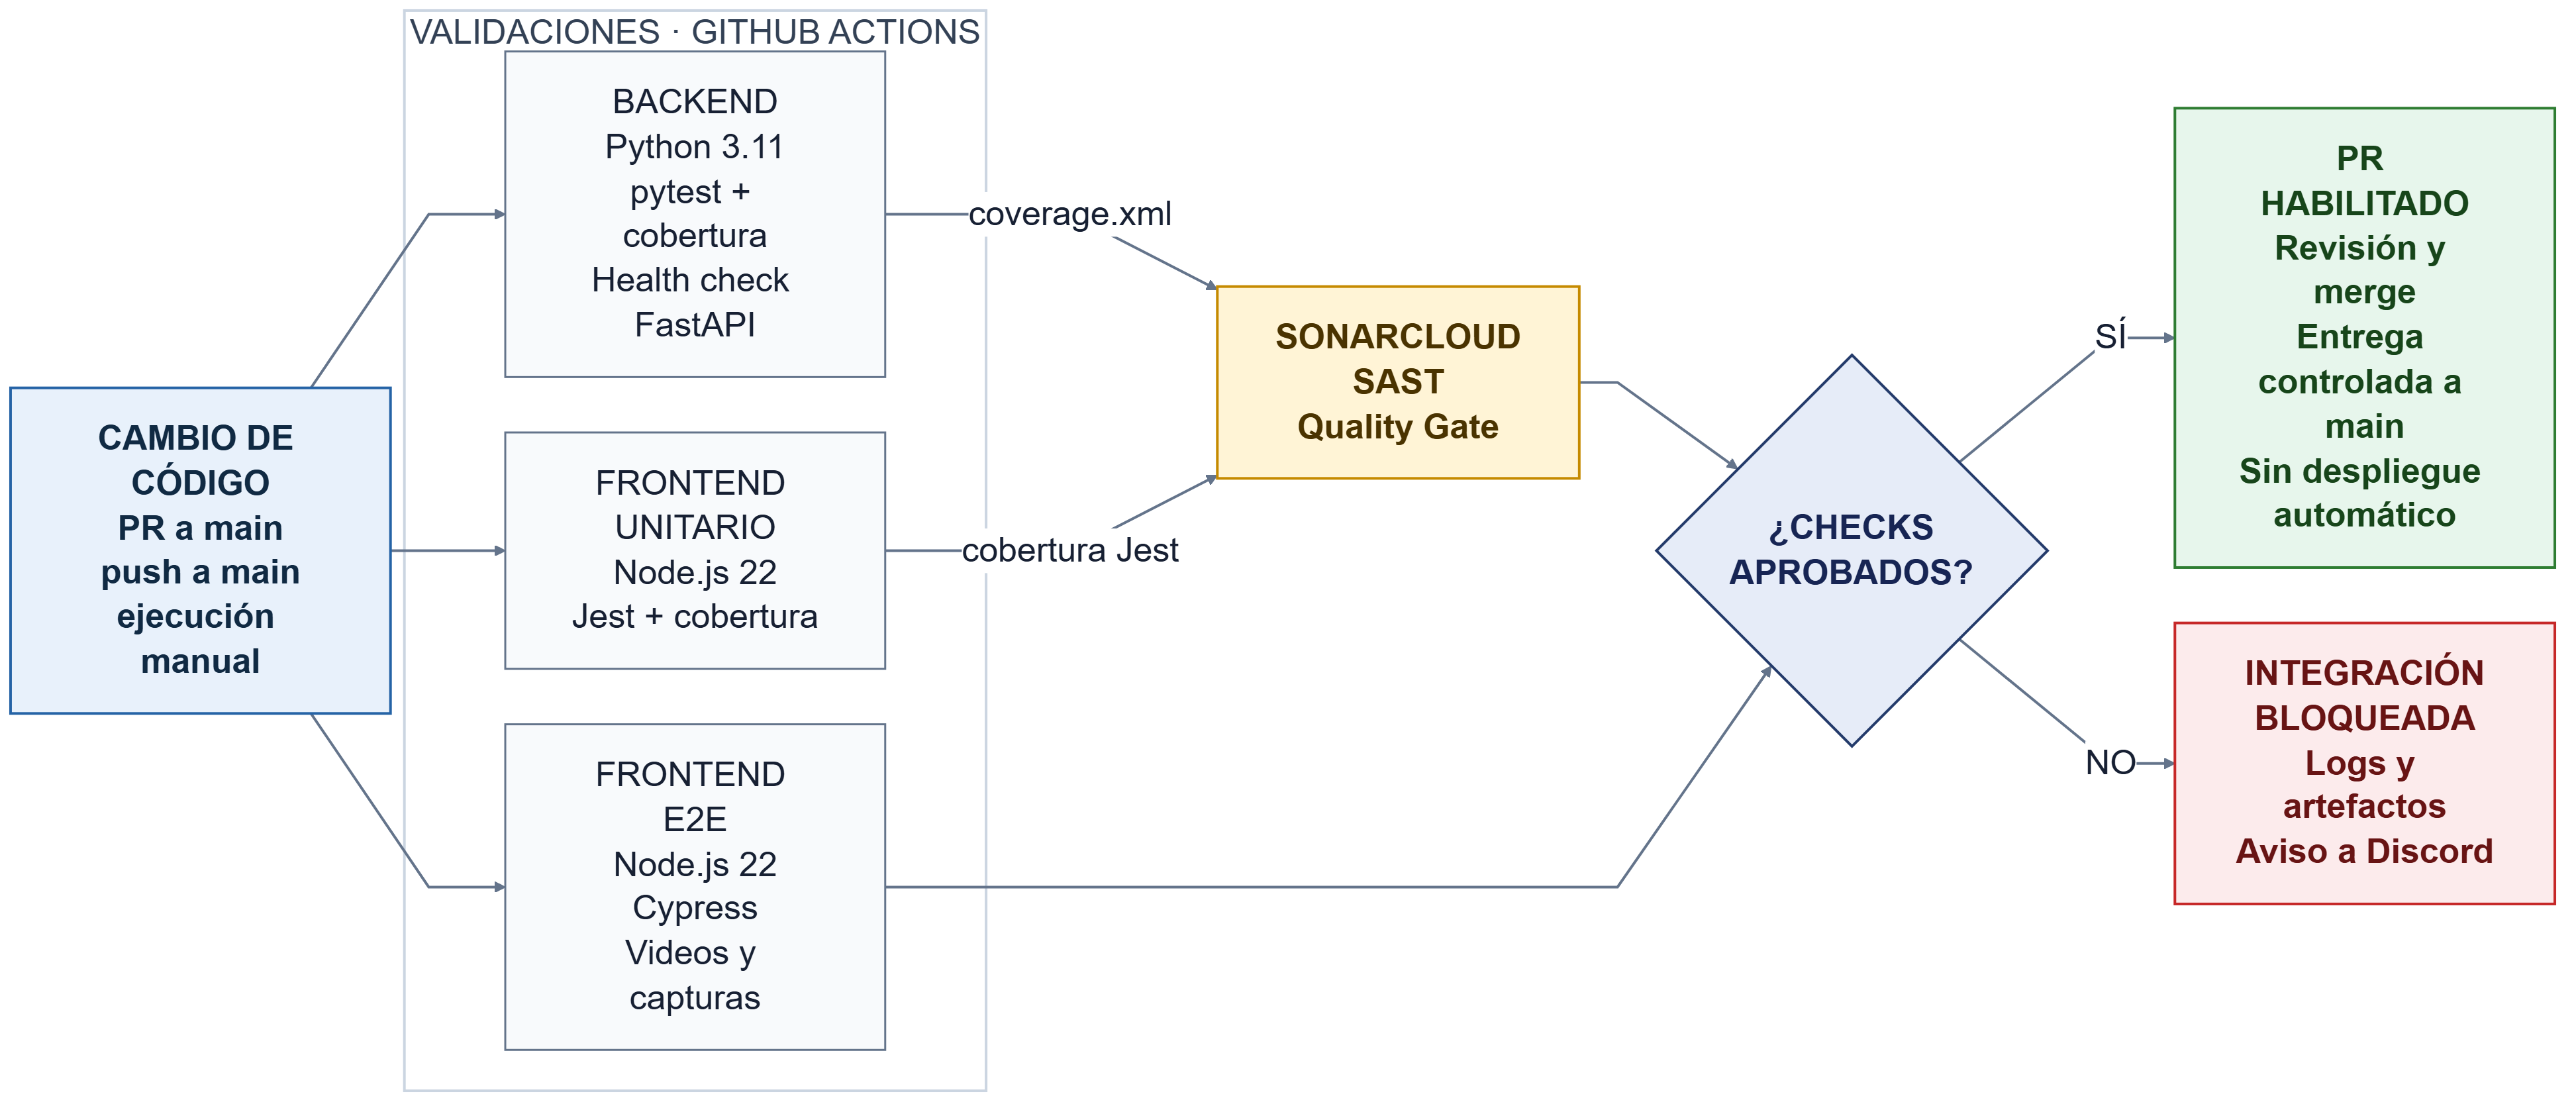
\includegraphics[width=0.98\linewidth]{imgs/pipeline-cicd-mermaid.png}
\caption{Diagrama Mermaid de alto nivel del pipeline CI/CD y DevSecOps de SpeechNotes}
\label{fig:pipeline-cicd}
\end{figure}
\end{landscape}

La Figura~\ref{fig:pipeline-cicd} presenta la arquitectura de alto nivel mediante un diagrama generado con Mermaid. Las pruebas de backend, las pruebas unitarias del frontend y las pruebas E2E se ejecutan como trabajos independientes. SonarCloud comienza únicamente cuando pytest y Jest concluyen correctamente, porque utiliza sus reportes de cobertura. Cypress se mantiene como un control paralelo de los flujos funcionales de la interfaz. El resultado conjunto de estos trabajos determina si el cambio puede continuar a revisión y mezcla.

\subsection{Etapas y evidencias}
\label{subsec:etapas-cicd}

\begingroup
\small
\begin{enumerate}
    \item \textbf{Pruebas de backend:} instala dependencias verificadas desde \texttt{requirements-test.lock}, inicia FastAPI en el puerto 9443, comprueba el endpoint \texttt{/health} y ejecuta pytest. Publica \texttt{coverage.xml} y el reporte JUnit \texttt{test-results.xml} como artefactos.
    \item \textbf{Pruebas unitarias del frontend:} instala dependencias reproducibles con \texttt{npm ci}, ejecuta Jest con cobertura y publica el directorio de evidencias generado.
    \item \textbf{Pruebas E2E:} ejecuta Cypress sobre la aplicación web y conserva videos y capturas, incluso cuando el trabajo falla, para facilitar el diagnóstico.
    \item \textbf{Análisis estático y seguridad:} descarga las coberturas de backend y frontend, ejecuta el escaneo de SonarCloud y espera hasta cinco minutos por la decisión del \textit{Quality Gate}. Esta etapa solo se ejecuta si pytest y Jest fueron exitosos.
    \item \textbf{Notificación y decisión:} cualquier fallo deja el check en rojo y envía una notificación a Discord con un enlace a la ejecución o al panel de SonarCloud. Con todos los checks aprobados, la protección de \texttt{main} permite continuar con la revisión y el merge del PR.
\end{enumerate}

El workflow implementa integración continua y una entrega controlada hasta la rama principal. Actualmente no contiene un trabajo de despliegue automático a producción; por tanto, la fase de despliegue permanece fuera de este pipeline y debe ejecutarse mediante el procedimiento operativo definido para el entorno de destino.
\endgroup

\chapter{Control de Medios y Suministros}
\label{sec:control-medios}

\section{Gestión de Artefactos}
\label{sec:artefactos}

Los artefactos evaluables del sprint SQA quedan consolidados en el presente informe. Para la entrega en GitHub se considera como artefacto documental final el SQAP generado desde el archivo principal de LaTeX; la matriz de rastreabilidad, los casos de prueba, el reporte de defectos, el análisis estático y el informe de cierre se integran como secciones y apéndices del mismo documento.

\begin{verbatim}
docs/
  sqa/
    speechNotes_sqap/            -- Informe SQAP final
      speechnotes_sqap.tex       -- Archivo principal
      secciones/                 -- Cuerpo del informe
      apendices/                 -- Matriz, casos, defectos y cierre
      imgs/                      -- Evidencias visuales usadas en el informe
      build.ps1                  -- Script de compilación
\end{verbatim}

\section{Control de Versiones}
\label{sec:versiones}

\begin{itemize}
    \item Los archivos LaTeX del informe se versionan en Git junto con el código fuente.
    \item Cada versión del SQAP se identifica por el tag del commit en Git.
    \item El PDF final del SQAP se etiqueta con el número de versión y fecha.
\end{itemize}

\chapter{Control de Proveedores}
\label{sec:proveedores}

\section{Proveedores Identificados}
\label{sec:proveedores-identificados}

La tabla~\ref{tab:proveedores} lista los proveedores externos utilizados en el proyecto.

\begin{longtable}{lll}
\caption{Proveedores externos}
\label{tab:proveedores}\\
\toprule
\textbf{Proveedor} & \textbf{Servicio} & \textbf{Dependencia}\\
\midrule
\endfirsthead
\toprule
\textbf{Proveedor} & \textbf{Servicio} & \textbf{Dependencia}\\
\midrule
\endhead
\bottomrule
\endfoot

NVIDIA NIM & Modelos de IA (ASR, BNR, VAD, Chat, Formatter) & Alta\\

MongoDB Atlas & Base de datos NoSQL en la nube & Alta\\

Vercel / Netlify & Despliegue de frontend & Media\\

Docker Hub & Imágenes de contenedores & Media\\

GitHub & Repositorio y CI/CD & Alta\\

Atlassian (Jira) & Gestión de incidencias & Baja\\

SonarCloud & Análisis estático & Media\\

\end{longtable}

\section{Criterios de Aceptación de Proveedores}
\label{sec:criterios-proveedores}

\begin{itemize}
    \item SLA definido y documentado.
    \item Compatibilidad con la arquitectura del proyecto.
    \item Disponibilidad de API pública documentada.
    \item Historial de uptime superior al 99\%.
\end{itemize}

\chapter{Registros y Actas}
\label{sec:registros}

\section{Registros Generados}
\label{sec:registros-generados}

Los siguientes registros fueron generados durante el sprint SQA:

\begin{longtable}{lp{5cm}p{5cm}}
\caption{Registros SQA}
\label{tab:registros}\\
\toprule
\textbf{Registro} & \textbf{Contenido} & \textbf{Ubicación}\\
\midrule
\endfirsthead
\toprule
\textbf{Registro} & \textbf{Contenido} & \textbf{Ubicación}\\
\midrule
\endhead
\bottomrule
\endfoot

Actas de reunión & Minutas de reuniones diarias (stand-ups) & Jira / docs\\

Reportes de prueba & Resultados de casos de prueba ejecutados & Apéndice~B\\

Reportes de defecto & Bugs encontrados durante la ejecución & Apéndice~C\\

Reporte SonarCloud & Análisis estático (antes/después) & Apéndice~D\\

Informe de cierre & Métricas y lecciones aprendidas & Apéndice~E\\

\end{longtable}

\section{Control de Registros}
\label{sec:control-registros}

\begin{itemize}
    \item Los registros electrónicos se almacenan en el repositorio Git (rama \texttt{planning-SQA}).
    \item El acceso está controlado por los permisos del repositorio GitHub.
    \item La retención mínima es de 1 año posterior a la entrega del proyecto.
\end{itemize}

\chapter{Capacitación}
\label{sec:capacitacion}

\section{Plan de Capacitación}
\label{sec:plan-capacitacion}

El equipo SQA recibió capacitación en las siguientes áreas antes del inicio del sprint:

\begin{longtable}{lp{4cm}p{6cm}}
\caption{Capacitación del equipo SQA}
\label{tab:capacitacion}\\
\toprule
\textbf{Área} & \textbf{Duración} & \textbf{Cobertura}\\
\midrule
\endfirsthead
\toprule
\textbf{Área} & \textbf{Duración} & \textbf{Cobertura}\\
\midrule
\endhead
\bottomrule
\endfoot

Jira Cloud & 2 h & Configuración de proyecto, tablero, issues, workflows\\

SonarCloud & 2 h & Análisis estático, calidad de código, reportes\\

pytest & 3 h & Pruebas unitarias, fixtures, mocks, httpx\\

Cypress & 3 h & Pruebas E2E, comandos personalizados, CI\\

Git & 1 h & Flujo de ramas, resolución de conflictos\\

LaTeX (Overleaf) & 1 h & Edición y compilación de documentos\\

\end{longtable}

\section{Capacitación Requerida}
\label{sec:capacitacion-requerida}

No se identificaron necesidades adicionales de capacitación para el equipo SQA durante este sprint. Para sprints futuros se recomienda capacitación en:

\begin{itemize}
    \item Pruebas de carga con k6 o Locust.
    \item Pruebas de seguridad con OWASP ZAP.
    \item Automatización de accesibilidad con axe-core.
\end{itemize}

\chapter{Gestión de Riesgos}
\label{sec:riesgos}

\section{Identificación y Categorización de Riesgos}
\label{sec:identificacion-riesgos}

Los riesgos asociados a la calidad de SpeechNotes se clasifican en dos categorías principales: \textbf{Riesgos del Producto} (asociados a la arquitectura, dependencias y comportamiento del software en producción) y \textbf{Riesgos del Proyecto de Pruebas} (asociados a la planificación, recursos y ejecución del sprint SQA).

\subsection{Riesgos del Producto (Software y Arquitectura)}
\label{subsec:riesgos-producto}

\begin{itemize}
    \item \textbf{RP-01: Caída o indisponibilidad de la API externa de NVIDIA NIM Cloud.}
    \begin{itemize}
        \item \textit{Probabilidad:} Media \quad \textit{Impacto:} Alto \quad \textit{Severidad:} Alta
        \item \textit{Plan de Mitigación:} Disponer de claves de API de respaldo y construir stubs/mocks desconectados en \texttt{pytest} para pruebas del backend sin dependencia externa.
    \end{itemize}
    \item \textbf{RP-02: Ausencia o falla en el dispositivo físico de entrada de audio (Micrófono).}
    \begin{itemize}
        \item \textit{Probabilidad:} Alta \quad \textit{Impacto:} Bajo \quad \textit{Severidad:} Media
        \item \textit{Plan de Mitigación:} Diseñar casos de prueba diferenciados (\texttt{CP-02}, \texttt{CP-15}) que validen la detección de entrada de audio y el manejo de errores por falta de permisos o hardware, complementando con simuladores de stream de audio en backend.
    \end{itemize}
    \item \textbf{RP-03: Inestabilidad o crasheos no controlados en la UI del frontend (React/Next.js).}
    \begin{itemize}
        \item \textit{Probabilidad:} Media \quad \textit{Impacto:} Medio \quad \textit{Severidad:} Media
        \item \textit{Plan de Mitigación:} Captura de logs de consola en Cypress y ejecución de pruebas exploratorias especificas para identificar pérdidas de estado en la UI.
    \end{itemize}
\end{itemize}

\subsection{Riesgos del Proyecto de Pruebas (Gestión y SQA)}
\label{subsec:riesgos-proyecto}

\begin{itemize}
    \item \textbf{RPJ-01: Tiempo insuficiente para completar automatización E2E al 100\%.}
    \begin{itemize}
        \item \textit{Probabilidad:} Alta \quad \textit{Impacto:} Medio \quad \textit{Severidad:} Alta
        \item \textit{Plan de Mitigación:} Adoptar una estrategia híbrida: priorizar la ejecución manual estructurada de los 17 casos de prueba críticos y automatizar únicamente los endpoints backend estables.
    \end{itemize}
    \item \textbf{RPJ-02: Discrepancias o problemas de compatibilidad en entornos locales de desarrollo.}
    \begin{itemize}
        \item \textit{Probabilidad:} Media \quad \textit{Impacto:} Alto \quad \textit{Severidad:} Alta
        \item \textit{Plan de Mitigación:} Utilizar la especificación de contenedores Docker (\texttt{docker-compose.yml}) y entornos virtuales unificados (\texttt{.venv}) para garantizar entornos replicables.
    \end{itemize}
    \item \textbf{RPJ-03: Documentación insuficiente de la API REST y eventos de WebSockets.}
    \begin{itemize}
        \item \textit{Probabilidad:} Baja \quad \textit{Impacto:} Alto \quad \textit{Severidad:} Media
        \item \textit{Plan de Mitigación:} Realizar sesiones de prueba exploratoria guiada y consultar directamente las especificaciones OpenAPI de FastAPI en \url{/docs}.
    \end{itemize}
\end{itemize}

\begin{longtable}{lllcp{4cm}}
\caption{Matriz consolidada de riesgos de Producto y Proyecto}
\label{tab:riesgos}\\
\toprule
\textbf{Código} & \textbf{Categoría} & \textbf{Prob / Imp} & \textbf{Severidad} & \textbf{Plan de Mitigación}\\
\midrule
\endfirsthead
\toprule
\textbf{Código} & \textbf{Categoría} & \textbf{Prob / Imp} & \textbf{Severidad} & \textbf{Plan de Mitigación}\\
\midrule
\endhead
\bottomrule
\endfoot

RP-01 & Producto & Media / Alto & Alta & Claves API respaldo y mocks en pytest\\

RP-02 & Producto & Alta / Bajo & Media & Casos de prueba de micrófono y permisos (CP-02, CP-15)\\

RP-03 & Producto & Media / Medio & Media & Captura de logs en Cypress e inspección\\

RPJ-01 & Proyecto & Alta / Medio & Alta & Estrategia híbrida (manual + pytest)\\

RPJ-02 & Proyecto & Media / Alto & Alta & Despliegue estandarizado con Docker\\

RPJ-03 & Proyecto & Baja / Alto & Media & Pruebas exploratorias sobre OpenAPI docs\\

\end{longtable}

\section{Resultados de Mitigación}
\label{sec:resultados-mitigacion}

\begin{itemize}
    \item \textbf{NVIDIA NIM (RP-01):} Se utilizó la clave de API activa de respaldo. Se completaron exitosamente las pruebas de formateo (\texttt{CP-09}), chat contextual (\texttt{CP-10}) y traducción (\texttt{CP-11}).
    \item \textbf{Inestabilidad frontend (RP-03):} Se identificó y aisló el defecto crítico \texttt{BUG-003} (crasheo del chat sin transcripción seleccionada), logrando su corrección antes del cierre del sprint.
    \item \textbf{Tiempo de automatización (RPJ-01):} Se garantizó el 100\% de ejecución manual de los 17 casos de prueba con soporte de scripts en \texttt{pytest}.
    \item \textbf{Micrófono (RP-02):} Se ejecutaron \texttt{CP-02} y \texttt{CP-15}, registrando detección de entrada de audio y manejo correcto de permisos denegados en la interfaz.
    \item \textbf{Manejo Global de Defectos:} Se registraron 8 defectos en Jira Software, logrando resolver el 100\% de los bloqueantes.
\end{itemize}

\begingroup\setlength{\tabcolsep}{0.5pt}\renewcommand{\arraystretch}{1.12}
\chapter{Alineación con ISO/IEC 25000 y Métricas de Calidad}
\label{sec:alineacion-iso-metricas}

\section{Objetivo, alcance y criterio de interpretación}

Este capítulo relaciona las prácticas y evidencias de SpeechNotes con la familia
ISO/IEC 25000 (SQuaRE) y con otras normas aplicables. El análisis cubre backend
Python/FastAPI, frontend Next.js/TypeScript, componentes de escritorio,
transcripción y funciones asistidas por inteligencia artificial.

La relación presentada constituye una evaluación de \textbf{alineación}; no es
una auditoría independiente, una certificación ISO ni una declaración formal de
conformidad. Los umbrales son criterios de aceptación definidos para SpeechNotes.
ISO/IEC 25023 propone medidas, pero no establece valores universales de aprobación.

\section{Resumen ejecutivo}

SpeechNotes dispone de requisitos trazables, casos positivos, negativos y de
límite, pruebas automatizadas, pruebas de extremo a extremo, análisis estático y
un \textit{Quality Gate} integrado en CI/CD. Sus principales puntos a favor son:

\begin{itemize}
    \item \textbf{Adecuación funcional:} los 19 requisitos funcionales de la matriz
    vigente tienen casos asociados. Se diseñaron 51 casos y cada requisito cuenta
    con entre 2 y 4 casos.
    \item \textbf{Mantenibilidad:} hay separación modular, pruebas unitarias y de
    integración, linting, SonarCloud, cobertura y dependencias bloqueadas.
    \item \textbf{Seguridad:} se evidencian autenticación, validación de rutas,
    variables de entorno, análisis estático y control del \textit{Quality Gate}.
    \item \textbf{Fiabilidad:} existen health checks y pruebas ante errores de
    WebSocket, entradas inválidas y fallos de proveedores.
    \item \textbf{Evaluación repetible:} GitHub Actions ejecuta pytest, Jest,
    Cypress y SonarCloud y conserva artefactos de prueba.
    \item \textbf{Base para evaluar IA:} los proveedores son sustituibles y se
    utilizan dobles de prueba. Faltan WER, fidelidad RAG y desempeño por idioma.
\end{itemize}

El cierre histórico es favorable en cobertura y análisis estático, pero la
verificación local del 22 de julio de 2026 encontró una falla en backend y otra
en frontend por falta de aislamiento del entorno. Tampoco existen series actuales
de latencia, disponibilidad, usabilidad o exactitud. La valoración global es de
\textbf{alineación parcial-alta con brechas de medición operativa y aislamiento}.

\section{Normas aplicables}

\begin{longtable}{p{3.4cm}p{5cm}p{6.2cm}}
\caption{Normas y relación con SpeechNotes}
\label{tab:normas-iso-speechnotes}\\
\toprule
\textbf{Norma} & \textbf{Aporte} & \textbf{Aplicación o evidencia}\\
\midrule
\endfirsthead
\toprule
\textbf{Norma} & \textbf{Aporte} & \textbf{Aplicación o evidencia}\\
\midrule
\endhead
\bottomrule
\endfoot
ISO/IEC 25000:2014 & Guía y vocabulario general de SQuaRE. & Ordena requisitos, modelos, medidas y evaluación.\\
ISO/IEC 25010:2023 & Modelo vigente de calidad con nueve características. & Base de la Tabla~\ref{tab:iso25010-evidencia}.\\
ISO/IEC 25023:2016 & Medición cuantitativa de calidad. & Base metodológica del catálogo; está en revisión a la fecha de corte.\\
ISO/IEC 25030:2019 & Gobierno de requisitos de calidad. & Cada métrica incluye fórmula, fuente, meta y responsable.\\
ISO/IEC 25040:2024 & Marco vigente de evaluación. & El SQAP conserva plan, criterios, resultados y evidencias.\\
ISO/IEC 25012:2008 & Modelo de calidad de datos. & Aplica a transcripciones, metadatos, documentos y embeddings.\\
ISO/IEC 25059:2023 & Modelo de calidad para IA. & Aplica a ASR, traducción, formateo y RAG.\\
ISO/IEC/IEEE 29119-2:2021 & Procesos de prueba. & Casos, matriz RF--CP, criterios, automatización y defectos.\\
ISO/IEC/IEEE 12207:2026 & Ciclo de vida del software. & Git, CI/CD, desarrollo, prueba y mantenimiento.\\
ISO/IEC 27001:2022 & Riesgos sobre confidencialidad, integridad y disponibilidad. & Hay controles técnicos, no evidencia de un SGSI completo.\\
ISO 9241-11:2018 & Usabilidad en contexto de uso. & Hay pruebas funcionales; faltan medidas con usuarios.\\
IEEE 730 & Procesos SQA. & El SQAP cita IEEE 730-1998, edición superada que debe actualizarse.\\
\end{longtable}

Fuentes oficiales consultadas el 22 de julio de 2026:
\url{https://www.iso.org/standard/64764.html},
\url{https://www.iso.org/standard/78176.html},
\url{https://www.iso.org/standard/35747.html},
\url{https://www.iso.org/standard/72116.html},
\url{https://www.iso.org/standard/83467.html},
\url{https://www.iso.org/standard/35736.html},
\url{https://www.iso.org/standard/80655.html},
\url{https://www.iso.org/standard/79428.html},
\url{https://www.iso.org/standard/90219.html},
\url{https://www.iso.org/standard/27001},
\url{https://www.iso.org/standard/63500.html} y
\url{https://standards.ieee.org/ieee/730/5284/}.

\section{Evaluación según ISO/IEC 25010:2023}

\begin{longtable}{p{3.2cm}p{6.9cm}p{2.2cm}p{3.8cm}}
\caption{Características ISO/IEC 25010:2023 y evidencia del proyecto}
\label{tab:iso25010-evidencia}\\
\toprule
\textbf{Característica} & \textbf{Puntos a favor} & \textbf{Estado} & \textbf{Evidencia}\\
\midrule
\endfirsthead
\toprule
\textbf{Característica} & \textbf{Puntos a favor} & \textbf{Estado} & \textbf{Evidencia}\\
\midrule
\endhead
\bottomrule
\endfoot
Adecuación funcional & Matriz RF--CP y 51 casos con caminos exitosos, errores y límites. & Fuerte & \path{docs/test/matriz_rastreabilidad.md} y casos de prueba.\\
Eficiencia de desempeño & Streaming, VAD y procesamiento por lotes. & No medida & Sin percentiles de latencia, capacidad o recursos.\\
Compatibilidad & REST, WebSocket, web, Electron, Tauri y proveedores encapsulados. & Parcial & \path{desktop/}, \path{web/src-tauri/} y protocolos NIM.\\
Capacidad de interacción & Login, dashboard, estados, visor, temas, zoom y mensajes. & Parcial & \path{web/app/}, E2E y capturas.\\
Fiabilidad & Salud, pérdida de WebSocket, entradas corruptas y fallos externos. & Parcial-fuerte & Pruebas de health, WebSocket y riesgos.\\
Seguridad & NextAuth, autenticación, rutas, SAST y \textit{Quality Gate}. & Parcial-fuerte & Auth, path security, SonarCloud y CI.\\
Mantenibilidad & Modularidad, patrones, linters, pruebas, cobertura y duplicación. & Fuerte con reservas & Suites y \path{sonar-project.properties}; revisar exclusiones.\\
Flexibilidad & Configuración por entorno, registro de proveedores y web/escritorio. & Parcial-fuerte & \path{.env.example}, NIM y factory de ambiente.\\
Seguridad operacional & Límites y manejo de errores; el dominio no se declara crítico. & No demostrada & Sin análisis de peligros por transcripciones incorrectas.\\
\end{longtable}

La principal fortaleza es la cadena requisito $\rightarrow$ caso $\rightarrow$
ejecución $\rightarrow$ defecto $\rightarrow$ corrección/reprueba $\rightarrow$
control automatizado. Un caso diseñado no equivale a ejecución y una captura
histórica no equivale al estado del commit actual.

\section{Línea base histórica y verificación actual}

\subsection{Evidencia histórica}

El Apéndice~\ref{apendice:e} registra 10 de 10 requisitos del alcance original,
17 de 17 casos manuales ejecutados, 13 aprobados y 4 fallidos. Reporta 8 defectos,
3 corregidos, 90.4\% de cobertura SonarCloud, 0.5\% de duplicación, seguridad A,
cero incidencias y \textit{Quality Gate} aprobado. Son cifras históricas, no una
medición reproducida en esta revisión.

La matriz vigente amplía el alcance documental a 19 requisitos y 51 casos: 34 de
camino exitoso, 13 de error y 4 de límite. Los 19 requisitos tienen casos. Esto
demuestra cobertura de \textbf{diseño}, no ejecución ni aprobación de los 51 casos.

\subsection{Ejecución local del 22 de julio de 2026}

\begin{table}[H]
\centering
\caption{Resultado de las suites ejecutadas durante la revisión}
\label{tab:ejecucion-actual-iso}
\begin{tabular}{lrrrrl}
\toprule
\textbf{Suite} & \textbf{Rec.} & \textbf{Aprob.} & \textbf{Fall.} & \textbf{Omit.} & \textbf{Tasa}\\
\midrule
Backend pytest & 362 & 251 & 1 & 110 & 99.60\%\\
Frontend Jest & 42 & 41 & 1 & 0 & 97.62\%\\
Consolidado & 404 & 292 & 2 & 110 & 99.32\%\\
\bottomrule
\end{tabular}
\end{table}

La tasa usa solo pruebas ejecutadas; las omitidas se informan aparte. Ambas suites
incumplen el criterio de suite verde. Las fallas se relacionaron con variables
sensibles heredadas: un test intentó contactar a un proveedor real y otro recibió
secretos que esperaba vacíos. Los valores no se reproducen. Si eran credenciales
reales, deben rotarse y los logs deben sanitizarse.

El backend local utilizó Python 3.14.3, mientras CI define Python 3.11. El comando
npm tampoco propagó la opción de cobertura al Jest interno; no se obtuvo una
cobertura frontend nueva y verificable.

\section{Catálogo documentado de métricas}

Cada medición debe registrar ID, objetivo, definición, fórmula, unidad, fuente,
commit, ambiente, responsable, fecha, umbral, resultado y decisión. Los estados
son: \textbf{cumple}, \textbf{no cumple}, \textbf{histórico} y
\textbf{no medido}.

\begin{landscape}
\small
\begin{longtable}{p{1cm}p{4.2cm}p{3.6cm}p{4.5cm}p{7.5cm}}
\caption{Definición, justificación, cumplimiento y evidencia de métricas}
\label{tab:catalogo-metricas-iso}\\
\toprule
\textbf{ID} & \textbf{Definición} & \textbf{Fórmula} & \textbf{Justificación y meta} & \textbf{Resultado, cumplimiento y evidencia}\\
\midrule
\endfirsthead
\toprule
\textbf{ID} & \textbf{Definición} & \textbf{Fórmula} & \textbf{Justificación y meta} & \textbf{Resultado, cumplimiento y evidencia}\\
\midrule
\endhead
\bottomrule
\endfoot
M-01 & RF con al menos un CP asociado. & $RF_c/RF_t\times100$ & Adecuación y trazabilidad. Meta 100\%. & 19/19 = 100\%. \textbf{Cumple}. Matriz RF--CP; no prueba ejecución.\\
M-02 & Menor cantidad de CP por RF. & $\min(CP\ por\ RF)$ & Evita cobertura nominal. Meta $\geq2$ y negativo/límite en funciones críticas. & Mínimo 2; 17/51 son error o límite. \textbf{Cumple parcialmente}; varios RF carecen de caso negativo.\\
M-03 & Aprobación backend sobre pruebas ejecutadas. & $P/(P+F+E)\times100$ & Fiabilidad. Meta CI 100\%. & 251/252 = 99.60\%; 110 omitidas. \textbf{No cumple}. Pytest 22/07/2026.\\
M-04 & Aprobación frontend sobre pruebas ejecutadas. & Igual a M-03. & Fiabilidad e interacción. Meta CI 100\%. & 41/42 = 97.62\%. \textbf{No cumple}. Jest 22/07/2026.\\
M-05 & Pruebas no omitidas sobre recolectadas. & $(P+F+E)/R\times100$ & Separa inventario de ejecución. Meta backend CI $\geq90$\%. & 252/362 = 69.61\%. \textbf{No cumple localmente}; repetir en CI con servicios.\\
M-06 & Cobertura de código instrumentado. & $cubiertos/medibles\times100$ & Mantenibilidad. Meta $\geq80$\% global y $\geq70$\% por componente crítico. & 90.4\% histórico. \textbf{Cumple históricamente; actual no verificado}. Apéndice~\ref{apendice:d}.\\
M-07 & Líneas duplicadas respecto del total. & $duplicadas/analizadas\times100$ & Modificabilidad. Meta $\leq3$\%. & 0.5\% histórico. \textbf{Cumple históricamente}. Apéndice~\ref{apendice:d}.\\
M-08 & Incidencias estáticas por severidad. & Conteo por severidad. & Seguridad y mantenibilidad. Meta: 0 críticas y 0 vulnerabilidades altas. & 0 incidencias y seguridad A históricas. \textbf{Cumple históricamente}; revisar exclusiones.\\
M-09 & Decisión del \textit{Quality Gate}. & Aprobado/rechazado. & Aceptación objetiva según 25040. Meta: aprobado. & Aprobado históricamente y workflow configurado. \textbf{Histórico/configurado}; vincular commit actual.\\
M-10 & Defectos cerrados y verificados. & $cerrados/encontrados\times100$ & Fiabilidad. Meta: 100\% críticos/mayores y $\geq80$\% total o riesgo aceptado. & 3/8 = 37.5\%; críticos 100\%, mayores 50\%. \textbf{No cumple global ni mayores; cumple críticos}.\\
M-11 & Latencia p95 de audio a texto parcial. & $P_{95}(t_{texto}-t_{audio})$ ms & Desempeño. Meta inicial p95 $\leq2000$ ms y error $<1$\%. & \textbf{No medido}. Instrumentar timestamps y reportar por sesión.\\
M-12 & Disponibilidad del servicio y flujo crítico. & $(T-indisponibilidad)/T\times100$ & Fiabilidad. Meta mensual $\geq99.5$\%. & \textbf{No medido}. Health check no demuestra disponibilidad mensual.\\
M-13 & Reconexiones WebSocket sin pérdida indebida. & $exitosas/simuladas\times100$ & Recuperabilidad. Meta $\geq99$\%. & \textbf{No medido}. Hay CP-008, CP-033 y tests, sin tasa.\\
M-14 & Exactitud ASR mediante WER. & $(S+D+I)/N\times100$ & Funcionalidad, IA y datos. Meta inicial audio limpio español $\leq15$\%. & \textbf{No medido}. Crear corpus versionado por ruido, acento e idioma.\\
M-15 & Respuestas RAG respaldadas por el documento. & $respaldadas/evaluadas\times100$ & Calidad IA. Meta $\geq95$\% y cero invenciones fuera de contexto. & \textbf{No medido}. Hay prompt y tests, no evaluación de contenido.\\
M-16 & Registros con metadatos obligatorios completos. & $completos/evaluados\times100$ & ISO 25012. Meta 100\%. & \textbf{No medido}. Usar repositorios, Prisma y pruebas de transcripción.\\
M-17 & Usuarios que completan tareas críticas. & $completan/participantes\times100$; tiempo y SUS & ISO 9241-11. Meta $\geq90$\% y SUS $\geq80$. & \textbf{No medido}. Evaluar login, grabación, transcripción, búsqueda y exportación.\\
M-18 & Tests aislados de secretos y red no simulada. & $aislados/tests\ de\ proveedor\times100$ & Seguridad y repetibilidad. Meta 100\%. & \textbf{No cumple cualitativamente}: dos fallas por entorno y una llamada externa. Falta inventariar denominador.\\
\end{longtable}
\normalsize
\end{landscape}

\section{Periodicidad y responsables}

\begin{longtable}{p{3.1cm}p{4cm}p{3.2cm}p{5.6cm}}
\caption{Programa de medición propuesto}
\label{tab:programa-medicion-iso}\\
\toprule
\textbf{Momento} & \textbf{Métricas} & \textbf{Responsable} & \textbf{Evidencia}\\
\midrule
\endfirsthead
\toprule
\textbf{Momento} & \textbf{Métricas} & \textbf{Responsable} & \textbf{Evidencia}\\
\midrule
\endhead
\bottomrule
\endfoot
Cada push/PR & M-03 a M-09 y M-18 & Desarrollo y QA & JUnit, cobertura, Sonar, logs sanitizados y SHA.\\
Cada sprint & M-01, M-02, M-10 y M-16 & QA Lead y Product Owner & Matriz RF--CP, defectos y reporte de datos.\\
Antes de liberar & M-03, M-04, M-08, M-09, M-10, M-14 y M-15 & Comité de aceptación & Acta con cumplimiento, excepciones y riesgo residual.\\
Operación mensual & M-11 a M-13 & Operaciones & Dashboard, incidentes y SLO.\\
Cambio de modelo/corpus/prompt & M-14 y M-15 & Responsable IA y QA & Dataset versionado y comparación con línea base.\\
\end{longtable}

\section{Brechas y acciones prioritarias}

\begin{enumerate}
    \item \textbf{Aislar pruebas y secretos:} usar configuración exclusiva para
    test, limpiar variables, bloquear red no simulada, sanitizar reportes y rotar
    credenciales reales expuestas.
    \item \textbf{Restablecer suites verdes:} corregir las dos fallas y ejecutar
    Python 3.11, Jest con cobertura y Cypress sobre el mismo commit.
    \item \textbf{Unificar alcance:} documentar el paso de 10 RF/17 CP históricos
    a 19 RF/51 CP actuales y registrar estado, fecha y evidencia por CP.
    \item \textbf{Medir el propósito central:} incorporar WER, latencia y fidelidad
    RAG para demostrar la calidad de transcripción y asistencia IA.
    \item \textbf{Definir SLO:} medir latencia p50/p95/p99, disponibilidad,
    errores, reconexión y recursos.
    \item \textbf{Evaluar usabilidad:} registrar éxito, tiempo, errores y
    satisfacción con usuarios representativos.
    \item \textbf{Revisar exclusiones Sonar:} asignar razón, responsable,
    caducidad y riesgo a cada exclusión.
    \item \textbf{Actualizar normas:} reemplazar IEEE 730-1998 por la referencia
    vigente o justificar formalmente la edición anterior.
\end{enumerate}

\section{Resumen para conferencia corta}

SpeechNotes combina captura de audio, detección de voz, transcripción en tiempo
real, traducción, búsqueda semántica y chat sobre documentos. El trabajo de
calidad construyó trazabilidad entre requisitos, casos, defectos y automatización.

ISO/IEC 25010 se utilizó como mapa de características; ISO/IEC 25023 para medidas;
ISO/IEC 25030 para requisitos cuantificables; e ISO/IEC 25040 para organizar la
evaluación. También se consideraron ISO/IEC 25059 para IA, ISO/IEC 25012 para los
datos, ISO/IEC/IEEE 29119 para pruebas e ISO/IEC 27001 para seguridad.

La matriz vigente cubre 19 requisitos con 51 casos diseñados. El cierre histórico
documenta 90.4\% de cobertura, 0.5\% de duplicación, seguridad A y \textit{Quality
Gate} aprobado. En la revisión actual, backend aprobó 251 de 252 pruebas ejecutadas
y frontend 41 de 42. Las fallas revelaron falta de aislamiento. También faltan
latencia, disponibilidad, usabilidad, WER y fidelidad de IA.

SpeechNotes no se presenta como producto certificado, sino como proyecto con
alineación práctica y evidencia verificable. El siguiente nivel de madurez es
mantener suites verdes, proteger secretos y actualizar métricas con fórmula,
umbral, responsable y evidencia por versión.

\section{Conclusión de cumplimiento}

M-01 cumple; M-02 cumple parcialmente; M-03, M-04, M-05, M-10 y M-18 no cumplen
al corte; M-06 a M-09 tienen cumplimiento histórico pendiente de reproducción; y
M-11 a M-17 no disponen de medición suficiente. El proyecto está bien encaminado
y respaldado por evidencia, pero no demuestra conformidad integral con ISO/IEC
25010 ni certificación bajo las normas citadas.

El catálogo debe mantenerse como parte viva del SQAP, actualizarse desde CI y
vincular cada resultado con commit, ambiente y artefacto.

\endgroup
\chapter{Pruebas de Rendimiento con Apache JMeter}
\label{sec:jmeter-rendimiento}

\section{Objetivo y alcance}

Se incorporó una prueba de carga HTTP reproducible para cubrir la brecha de
eficiencia de desempeño identificada en el Capítulo~\ref{sec:alineacion-iso-metricas}.
El plan verifica los endpoints \path{/health} y \path{/} con usuarios virtuales,
rampa e iteraciones parametrizables. Esta prueba aporta evidencia a ISO/IEC
25010:2023 (eficiencia de desempeño y fiabilidad), ISO/IEC 25023:2016 (medición)
e ISO/IEC 25040:2024 (evaluación y criterios de aceptación).

\textbf{Estado al cierre de este documento: codificada y no ejecutada.} No se
declara cumplimiento de rendimiento hasta disponer de un JTL generado por CI.

\section{Diseño de la prueba}

\begin{table}[H]
\centering
\caption{Configuración predeterminada del plan JMeter}
\label{tab:jmeter-configuracion}
\begin{tabular}{p{4.3cm}p{4cm}p{6cm}}
\toprule
\textbf{Parámetro} & \textbf{Valor por defecto} & \textbf{Propósito}\\
\midrule
Usuarios concurrentes & 10 & Simular concurrencia controlada.\\
Rampa & 10 segundos & Evitar inicio instantáneo artificial.\\
Iteraciones por usuario & 5 & Producir 100 muestras entre dos endpoints.\\
Pausa entre solicitudes & 100 ms & Evitar un bucle sin tiempo de pensamiento.\\
Timeout de conexión & 3000 ms & Limitar conexiones bloqueadas.\\
Timeout de respuesta & 5000 ms & Limitar solicitudes sin respuesta.\\
\bottomrule
\end{tabular}
\end{table}

El archivo \path{tests/performance/speechnotes-load-test.jmx} no contiene claves,
tokens ni datos personales. Cada sampler exige código HTTP 200. El host, puerto,
protocolo, hilos, rampa, iteraciones y timeouts se inyectan mediante propiedades
\texttt{-J}, lo que permite mantener el mismo plan entre local y CI.

\section{Métricas, definición y criterios de cumplimiento}

\begin{longtable}{p{2cm}p{4.2cm}p{3.4cm}p{5.6cm}}
\caption{Métricas del control de rendimiento}
\label{tab:jmeter-metricas}\\
\toprule
\textbf{ID} & \textbf{Definición y fórmula} & \textbf{Meta} & \textbf{Justificación, cumplimiento y evidencia}\\
\midrule
\endfirsthead
\toprule
\textbf{ID} & \textbf{Definición y fórmula} & \textbf{Meta} & \textbf{Justificación, cumplimiento y evidencia}\\
\midrule
\endhead
\bottomrule
\endfoot
JM-01 & Cantidad de muestras válidas registradas en JTL. & $\geq 100$ & Evita aprobar una ejecución incompleta. \textbf{No medido}; evidencia futura: \path{results.jtl}.\\
JM-02 & Tasa de error: $muestras\ fallidas / muestras\ totales \times 100$. & $\leq 1\%$ & Mide fiabilidad bajo carga. \textbf{No medido}; se evalúa automáticamente.\\
JM-03 & Latencia p95: percentil 95 de \texttt{elapsed}. & $\leq 2000$ ms & Controla la experiencia de la mayoría de solicitudes sin ocultar la cola. \textbf{No medido}.\\
JM-04 & Throughput: solicitudes completadas por segundo. & Línea base, sin gate inicial & Permite comparar tendencias entre commits. \textbf{No medido}; se reporta en HTML.\\
\end{longtable}

El script \path{scripts/evaluate_jmeter_results.py} procesa el JTL con la librería
estándar de Python y devuelve código distinto de cero si JM-01, JM-02 o JM-03 no
cumplen. Los umbrales son iniciales y deben revisarse después de obtener una línea
base estable en un runner controlado.

\section{Integración en CI/CD y evidencia}

El workflow \path{.github/workflows/jmeter-performance.yml} se activa en push y
pull request hacia \texttt{main}, además de ejecución manual. Sus pasos son:

\begin{enumerate}
    \item instalar dependencias reproducibles del backend con Python 3.11;
    \item iniciar FastAPI y esperar el health check;
    \item ejecutar JMeter 5.6.3 en modo no gráfico mediante contenedor;
    \item evaluar automáticamente muestras, errores y p95;
    \item publicar JTL, reporte HTML y log del backend durante 14 días;
    \item detener el backend incluso cuando falle un paso.
\end{enumerate}

El job tiene límite de 15 minutos, permisos de solo lectura y cancelación de
ejecuciones anteriores de la misma rama. El reporte se conserva como artefacto
\texttt{jmeter-performance-report}. El gate complementa pytest, Jest, Cypress y
SonarCloud; no reemplaza pruebas funcionales ni observabilidad de producción.

\section{Cómo ejecutar en el futuro}

La ejecución manual puede parametrizar usuarios e iteraciones desde
\textit{workflow\_dispatch}. Para una prueba local equivalente se requiere iniciar
el backend en el puerto 9443 y ejecutar JMeter 5.6.3 en modo no gráfico contra el
JMX. Por instrucción del alcance actual, \textbf{la prueba no fue ejecutada durante
esta actualización}; únicamente se codificó, integró y documentó.

\chapter{Conclusiones}
\label{sec:conclusiones}

\section{Desempeño General}
\label{sec:desempenio-general}

El sprint de calidad de SpeechNotes se ejecutó conforme al plan establecido, con una cobertura del 100\% de los requisitos funcionales y una tasa de aprobación del 76.47\% en los casos de prueba ejecutados. CP-09 quedó aprobado después de la corrección y re-prueba; CP-05 y CP-16 mantienen fallas funcionales evidenciadas que requieren seguimiento.

\section{Hallazgos Clave}
\label{sec:hallazgos-clave}

\begin{enumerate}
    \item \textbf{Funcionalidad Core Evaluada:} Los requisitos de autenticación, captura, transcripción, consulta, búsqueda, IA, traducción y chat quedaron cubiertos. RF-03, RF-05 y RF-07 mantienen fallas documentadas; el formateo IA de RF-09 se recuperó después de corregir el WebSocket y la selección de modelos disponibles.

    \item \textbf{Problemas de UX Detectados:} Se identificaron defectos menores de experiencia de usuario en autenticación, grabación y carga de archivos; los abiertos quedaron registrados para seguimiento sin bloquear los flujos principales.

    \item \textbf{Mejora Significativa en Calidad de Código:} El análisis final de SonarCloud registró 90.4\% de cobertura, 0 issues abiertos, Security Rating A, 0 issues de seguridad, 0.5\% de duplicación y \textit{Quality Gate} aprobado.

    \item \textbf{Automatización como Inversión:} Las suites de pytest y Cypress configuradas proporcionan una base sólida para regression testing en sprints futuros.

    \item \textbf{Bugs Identificados:} Se encontraron 8 bugs (3 corregidos, 5 pendientes). El bug crítico fue corregido durante el sprint. Quedan 5 defectos pendientes, incluido BUG-005 de severidad Major, registrados para el siguiente ciclo de remediación.
\end{enumerate}

\section{Recomendaciones}
\label{sec:recomendaciones}

\begin{enumerate}
    \item \textbf{Corregir bugs pendientes:} Los 5 bugs abiertos deben ser atendidos en el siguiente sprint de desarrollo.
    \item \textbf{Pruebas de carga:} Realizar pruebas de carga formal con k6 o Locust para validar el comportamiento bajo estrés.
    \item \textbf{Documentación de API:} Completar la documentación de los endpoints REST de la API.
    \item \textbf{Pruebas de seguridad:} Integrar OWASP ZAP en el pipeline CI/CD.
    \item \textbf{Monitoreo de SonarCloud:} Mantener el quality gate activo en el pipeline de CI/CD para prevenir regresiones.
    \item \textbf{Ampliar automatización:} Incrementar la cobertura de pruebas automatizadas, especialmente en flujos de error y casos límite.
    \item \textbf{Mejoras de UX:} Implementar tooltip contextual en lugar del modal de error de micrófono.
\end{enumerate}

\section{Lecciones Aprendidas}
\label{sec:lecciones}

\begin{enumerate}
    \item La planificación detallada (matriz de rastreabilidad, casos de prueba) antes de la ejecución redujo significativamente la ambigüedad durante las pruebas.
    \item La integración temprana de SonarCloud permitió detectar code smells antes de que se acumularan.
    \item El uso de Jira para el seguimiento de bugs facilitó la comunicación entre QA y desarrollo.
    \item Para sprints futuros, se recomienda asignar tiempo adicional para pruebas exploratorias y de accesibilidad.
\end{enumerate}

\appendix
\chapter{Matriz de Rastreabilidad}
\label{apendice:a}

\section{Cobertura de Requisitos vs. Casos de Prueba}

La siguiente matriz consolida la trazabilidad del sprint SQA dentro de este informe. Cada requisito funcional queda asociado con sus casos de prueba ejecutados, el resultado consolidado y los defectos vinculados cuando aplica.

\begin{landscape}
\begin{longtable}{p{1.4cm}p{5.2cm}p{4.6cm}p{3cm}p{4.6cm}}
\caption{Matriz de rastreabilidad de requisitos funcionales vs. casos de prueba}
\label{tab:matriz-rastreabilidad}\\
\toprule
\textbf{RF} & \textbf{Requisito evaluado} & \textbf{Caso(s) de prueba} & \textbf{Resultado} & \textbf{Defectos asociados}\\
\midrule
\endfirsthead
\toprule
\textbf{RF} & \textbf{Requisito evaluado} & \textbf{Caso(s) de prueba} & \textbf{Resultado} & \textbf{Defectos asociados}\\
\midrule
\endhead
\bottomrule
\endfoot

RF-01 & Auth (autenticación y sesiones) & CP-01 Login demo; CP-14 credenciales incorrectas; CP-17 bloqueo de rutas administrativas & \textcolor{PasoColor}{Pasado con observaciones} & BUG-006 y BUG-008 abiertos, severidad Minor\\
RF-02 & Audio / Frontend (captura de dispositivo) & CP-02 prueba de micrófono; CP-15 denegación de permisos & \textcolor{PasoColor}{Pasado} & No aplica\\
RF-03 & Audio / Backend (procesamiento VAD) & CP-03 iniciar/detener grabación; CP-12 configuración VAD & \textcolor{FalloColor}{Fallado parcial} & BUG-002 abierto y BUG-007 cerrado, severidad Minor\\
RF-04 & Realtime ASR (transcripción en vivo) & CP-04 transcripción en vivo & \textcolor{PasoColor}{Pasado} & No aplica\\
RF-05 & Upload / Backend (ingesta de audio) & CP-05 upload de audio; CP-16 formato inválido & \textcolor{FalloColor}{Fallado} & Dos incidencias funcionales abiertas; BUG-009 permanece como observación Minor\\
RF-06 & Transcripciones (persistencia y consulta) & CP-06 consultar transcripciones; CP-13 eliminar transcripción & \textcolor{PasoColor}{Pasado} & No aplica\\
RF-07 & Editor (edición de contenido) & CP-07 editar y guardar transcripción & \textcolor{FalloColor}{Fallado} & BUG-004 cerrado y BUG-005 abierto, severidad Major\\
RF-08 & Búsqueda (búsqueda textual) & CP-08 buscar dentro de transcripciones & \textcolor{PasoColor}{Pasado} & No aplica\\
RF-09 & IA / Formatter (estructuración con LLM) & CP-09 formateo IA; CP-11 traducción de transcripción & \textcolor{PasoColor}{Pasado en re-prueba} & CP-09 falló inicialmente y fue corregido tras registrar la incidencia\\
RF-10 & Chat / RAG (asistente contextual) & CP-10 chat contextual sobre una nota & \textcolor{PasoColor}{Pasado con defecto cerrado} & BUG-003 cerrado, severidad Critical\\

\bottomrule
\end{longtable}
\end{landscape}

\section{Detalle de Ejecución por Caso de Prueba}

\begin{longtable}{p{1.6cm}p{1.6cm}p{6.2cm}p{2.4cm}p{4.8cm}}
\caption{Trazabilidad de casos de prueba, resultados y defectos}
\label{tab:trazabilidad-casos}\\
\toprule
\textbf{CP} & \textbf{RF} & \textbf{Caso de prueba} & \textbf{Estado} & \textbf{Defecto asociado}\\
\midrule
\endfirsthead
\toprule
\textbf{CP} & \textbf{RF} & \textbf{Caso de prueba} & \textbf{Estado} & \textbf{Defecto asociado}\\
\midrule
\endhead
\bottomrule
\endfoot

CP-01 & RF-01 & Login con usuario demo & \textcolor{PasoColor}{Pasado} & No aplica\\
CP-02 & RF-02 & Prueba de micrófono & \textcolor{PasoColor}{Pasado} & No aplica\\
CP-03 & RF-03 & Iniciar y detener grabación & \textcolor{FalloColor}{Fallado} & BUG-002 abierto\\
CP-04 & RF-04 & Transcripción en vivo & \textcolor{PasoColor}{Pasado} & No aplica\\
CP-05 & RF-05 & Upload de audio para transcribir & \textcolor{FalloColor}{Fallado} & No se genera la transcripción; incidencia abierta\\
CP-06 & RF-06 & Consultar transcripciones guardadas & \textcolor{PasoColor}{Pasado} & No aplica\\
CP-07 & RF-07 & Editar y guardar una transcripción & \textcolor{FalloColor}{Fallado} & BUG-005 abierto\\
CP-08 & RF-08 & Buscar dentro de transcripciones & \textcolor{PasoColor}{Pasado} & No aplica\\
CP-09 & RF-09 & Formateo IA de una transcripción & \textcolor{PasoColor}{Pasado en re-prueba} & Incidencia corregida: WebSocket, modelos y persistencia\\
CP-10 & RF-10 & Chat contextual sobre una nota & \textcolor{PasoColor}{Pasado} & BUG-003 cerrado\\
CP-11 & RF-09 & Traducción de transcripción & \textcolor{PasoColor}{Pasado} & No aplica\\
CP-12 & RF-03 & Modificar configuraciones VAD & \textcolor{PasoColor}{Pasado} & BUG-007 cerrado como observación histórica\\
CP-13 & RF-06 & Eliminar transcripción & \textcolor{PasoColor}{Pasado} & No aplica\\
CP-14 & RF-01 & Login con credenciales incorrectas & \textcolor{PasoColor}{Pasado} & No aplica\\
CP-15 & RF-02 & Denegación de permisos de micrófono & \textcolor{PasoColor}{Pasado} & No aplica\\
CP-16 & RF-05 & Upload de formato inválido & \textcolor{FalloColor}{Fallado} & Validación de formato en UI pendiente\\
CP-17 & RF-01 & Bloqueo de rutas administrativas & \textcolor{PasoColor}{Pasado} & No aplica\\

\bottomrule
\end{longtable}

\section{Resumen de Cobertura}

\begin{itemize}
    \item Total de requisitos funcionales: 10
    \item Requisitos cubiertos por al menos un caso de prueba: 10 (100\%)
    \item Total de casos de prueba ejecutados: 17
    \item Casos pasados: 13 (76.47\%), incluido CP-09 aprobado en re-prueba
    \item Casos fallados: 4 (23.53\%)
    \item Defectos con identificador formal registrados: 8
    \item Incidencias de flujos críticos evidenciadas: 3 (1 resuelta y 2 pendientes)
    \item Defectos corregidos: 3 (37.5\%)
    \item Defectos abiertos: 5 (62.5\%)
    \item Defectos críticos abiertos al cierre: 0
\end{itemize}

\chapter{Casos de Prueba}
\label{apendice:b}

\section{Casos de Prueba Manuales}

Los 17 casos de prueba definidos para el sprint fueron registrados y organizados en Zephyr Advanced. La Figura~\ref{fig:zephyr-casos-prueba} muestra el catálogo completo utilizado como base para la ejecución manual y la trazabilidad con los requisitos funcionales.

\begin{figure}[H]
\centering
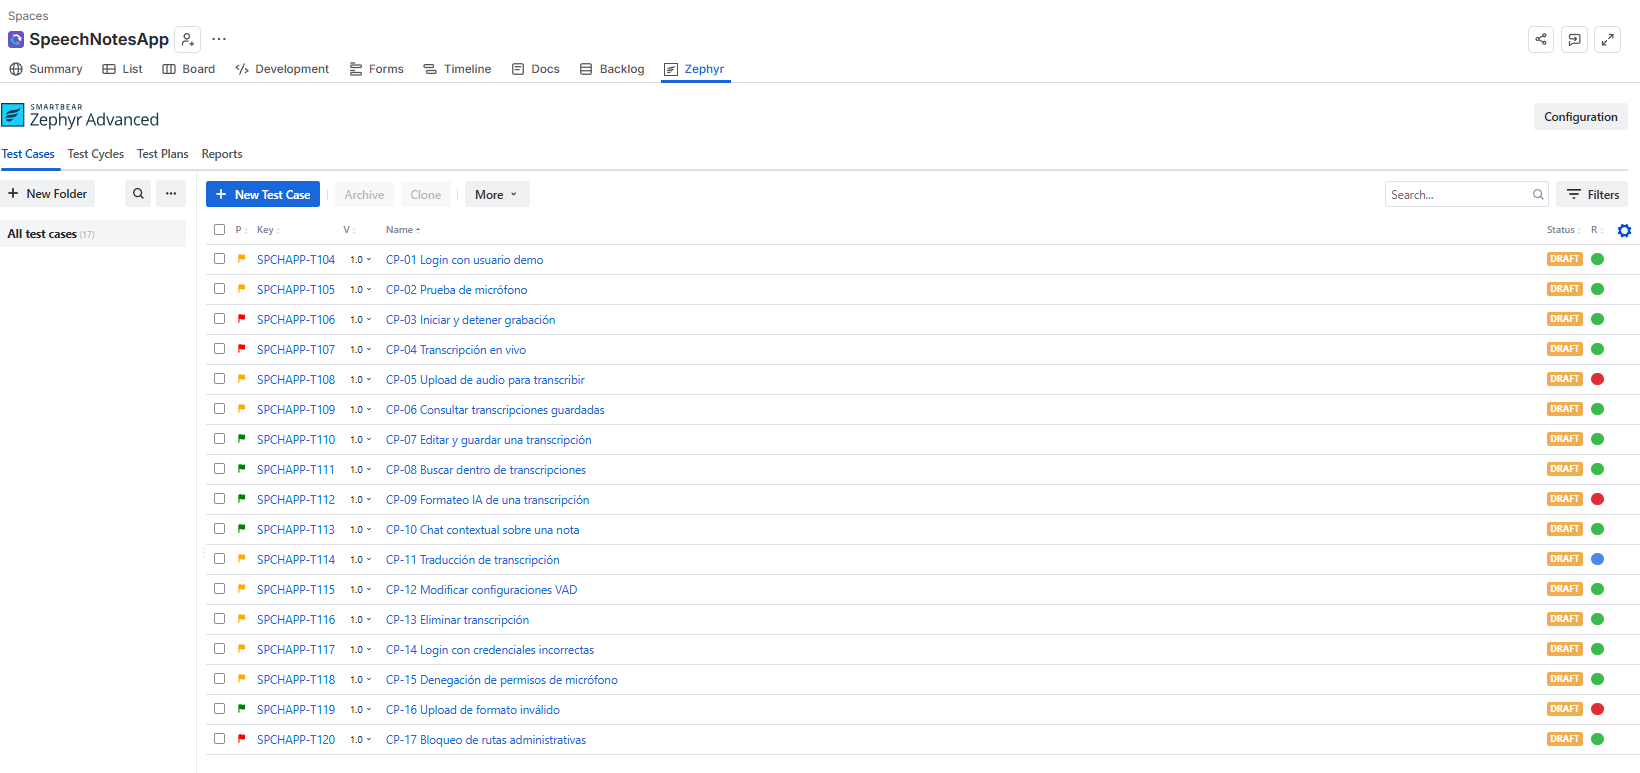
\includegraphics[width=\textwidth]{../../informe/images/zephyr-test-cases.png}
\caption{Catálogo de 17 casos de prueba registrado en Zephyr Advanced}
\label{fig:zephyr-casos-prueba}
\end{figure}

\subsection{CP-01: Login con usuario demo}
\label{cp:01}

\begin{longtable}{lp{10cm}}
\toprule
\textbf{Campo} & \textbf{Valor}\\
\midrule
\endhead
\bottomrule
\endfoot

\textbf{ID} & CP-01\\
\textbf{Objetivo} & Validar acceso de usuario de pruebas\\
\textbf{Título} & Login con usuario demo\\
\textbf{Precondiciones} & Frontend en 3006 y Backend en 9443\\
\textbf{Pasos} & 1) Abrir http://localhost:3006/login. 2) Ingresar correo demo@speechnotes.app y password demo123. 3) Presionar el botón de inicio de sesión.\\
\textbf{Resultado Esperado} & 1) Se muestra la pantalla de inicio de sesión. 2) Los campos se llenan correctamente. 3) El usuario es redirigido a /dashboard exitosamente.\\
\textbf{Resultado Obtenido} & OK\\
\textbf{Estado} & \textcolor{PasoColor}{Pasado}\\
\bottomrule
\end{longtable}

\begin{figure}[H]
\centering
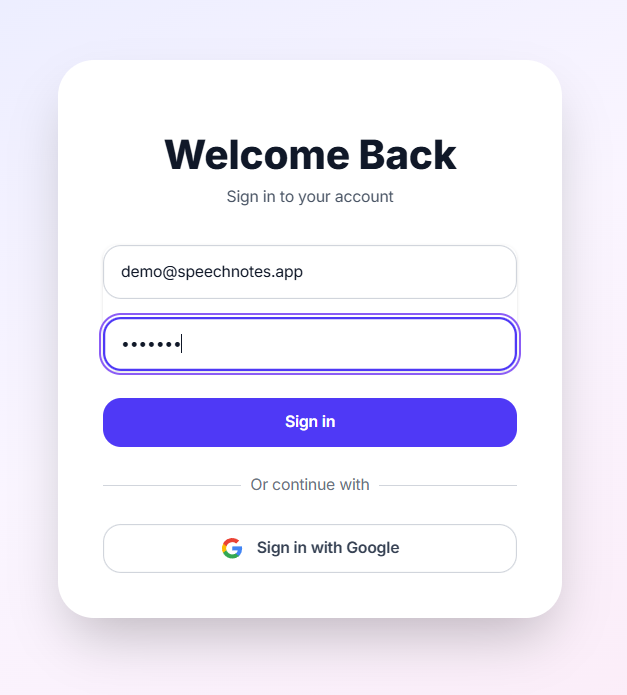
\includegraphics[width=0.55\textwidth]{imgs/login.png}
\caption{CP-01: Login con usuario demo - login.png}
\label{fig:cp01_login}
\end{figure}

\begin{figure}[H]
\centering
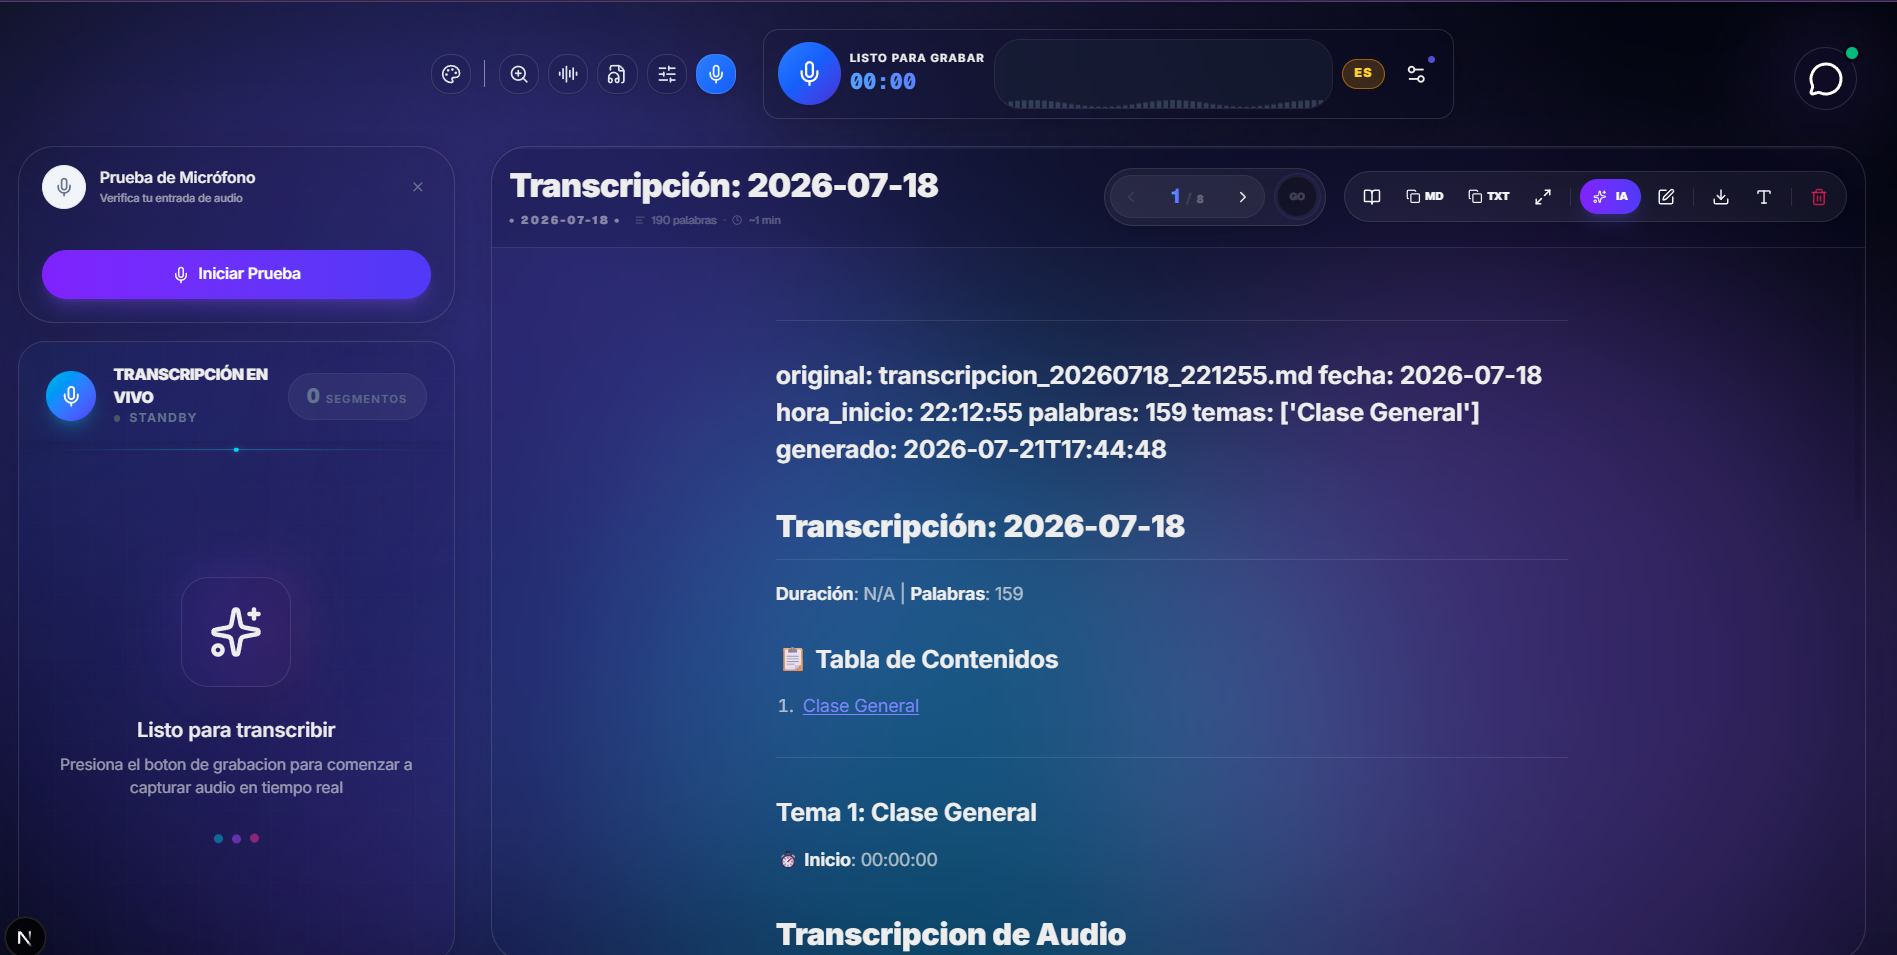
\includegraphics[width=0.55\textwidth]{imgs/dashboard.png}
\caption{CP-01: Login con usuario demo - dashboard.png}
\label{fig:cp01_dashboard}
\end{figure}

\subsection{CP-02: Prueba de micrófono}
\label{cp:02}

\begin{longtable}{lp{10cm}}
\toprule
\textbf{Campo} & \textbf{Valor}\\
\midrule
\endhead
\bottomrule
\endfoot

\textbf{ID} & CP-02\\
\textbf{Objetivo} & Asegurar que el sistema detecta entrada de audio\\
\textbf{Título} & Prueba de micrófono\\
\textbf{Precondiciones} & Micrófono conectado\\
\textbf{Pasos} & 1) Abrir http://localhost:3006/login. 2) Ingresar credenciales válidas y presionar inicio de sesión. 3) Navegar a la opción de Prueba de Micrófono. 4) Otorgar permisos de micrófono en el prompt del navegador. 5) Hablar al micrófono de forma continua por 5 a 10 segundos.\\
\textbf{Resultado Esperado} & 1) Carga la pantalla de inicio de sesión. 2) Redirección exitosa al Dashboard. 3) Se muestra la interfaz de prueba de audio. 4) Se habilita el acceso al dispositivo de entrada. 5) El indicador visual responde y muestra actividad.\\
\textbf{Resultado Obtenido} & OK\\
\textbf{Estado} & \textcolor{PasoColor}{Pasado}\\
\bottomrule
\end{longtable}

\begin{figure}[H]
\centering
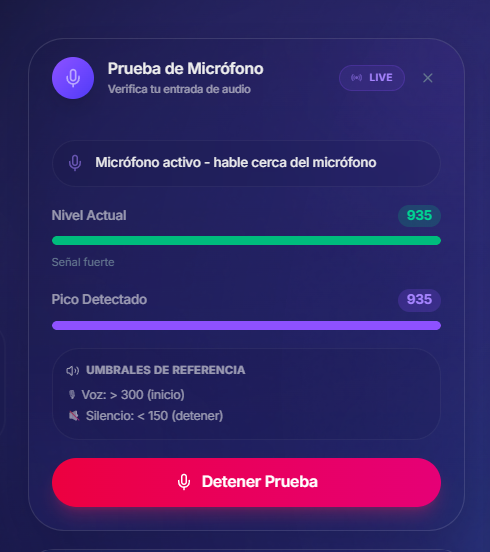
\includegraphics[width=0.55\textwidth]{imgs/prueba-mic.png}
\caption{CP-02: Prueba de micrófono - prueba-mic.png}
\label{fig:cp02_prueba-mic}
\end{figure}

\subsection{CP-03: Iniciar y detener grabación}
\label{cp:03}

\begin{longtable}{lp{10cm}}
\toprule
\textbf{Campo} & \textbf{Valor}\\
\midrule
\endhead
\bottomrule
\endfoot

\textbf{ID} & CP-03\\
\textbf{Objetivo} & Verificar la captura y envío de audio\\
\textbf{Título} & Iniciar y detener grabación\\
\textbf{Precondiciones} & Micrófono configurado\\
\textbf{Pasos} & 1) Abrir http://localhost:3006/login. 2) Ingresar credenciales válidas y presionar inicio de sesión. 3) En el Dashboard presionar el botón principal de Iniciar grabación. 4) Hablar al micrófono durante al menos 10 segundos. 5) Presionar el botón de Detener y confirmar la detención. 6) Esperar a que termine el procesamiento.\\
\textbf{Resultado Esperado} & 1) Carga la pantalla de inicio de sesión. 2) Redirección exitosa al Dashboard. 3) La interfaz cambia a estado grabando. 4) El audio es capturado correctamente. 5) El sistema muestra estado de procesamiento. 6) Se genera una nueva nota en la lista de transcripciones.\\
\textbf{Resultado Obtenido} & Falla en consola: No se encontró la referencia (BUG-002)\\
\textbf{Estado} & \textcolor{FalloColor}{Fallado}\\
\bottomrule
\end{longtable}

\begin{figure}[H]
\centering

\includegraphics[width=0.55\textwidth]{imgs/grabar.png}
\caption{CP-03: Iniciar y detener grabación - grabar.png}
\label{fig:cp03_grabar}
\end{figure}

\begin{figure}[H]
\centering
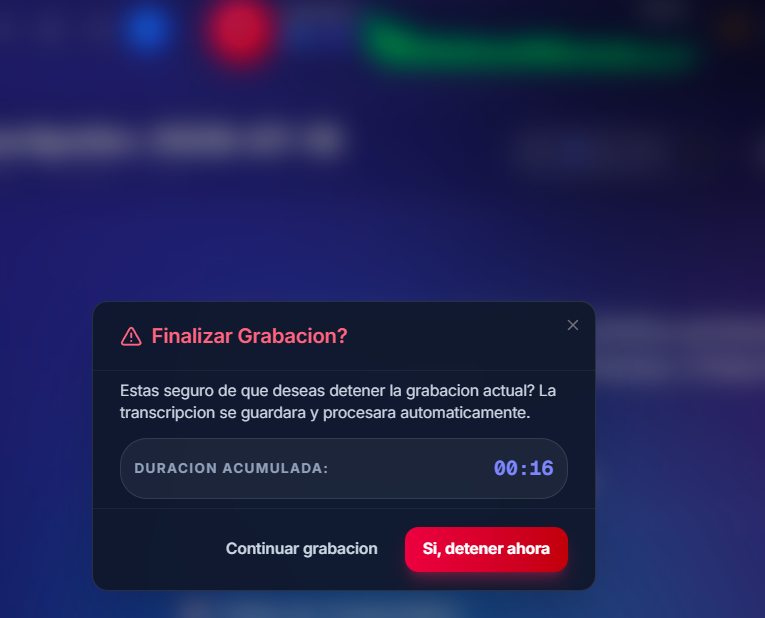
\includegraphics[width=0.55\textwidth]{imgs/stop.png}
\caption{CP-03: Iniciar y detener grabación - stop.png}
\label{fig:cp03_stop}
\end{figure}

\subsection{CP-04: Transcripción en vivo}
\label{cp:04}

\begin{longtable}{lp{10cm}}
\toprule
\textbf{Campo} & \textbf{Valor}\\
\midrule
\endhead
\bottomrule
\endfoot

\textbf{ID} & CP-04\\
\textbf{Objetivo} & Validar recepción de texto mediante WebSockets\\
\textbf{Título} & Transcripción en vivo\\
\textbf{Precondiciones} & Servidor ASR activo\\
\textbf{Pasos} & 1) Abrir http://localhost:3006/login. 2) Ingresar credenciales válidas y presionar inicio de sesión. 3) En el Dashboard iniciar una grabación de audio. 4) Hablar oraciones claras de forma constante durante 30 segundos. 5) Detener la grabación.\\
\textbf{Resultado Esperado} & 1) Carga la pantalla de inicio de sesión. 2) Redirección exitosa al Dashboard. 3) El micrófono comienza a capturar datos. 4) Aparecen segmentos de texto en vivo en la pantalla. 5) El texto final se consolida sin duplicarse incorrectamente.\\
\textbf{Resultado Obtenido} & OK\\
\textbf{Estado} & \textcolor{PasoColor}{Pasado}\\
\bottomrule
\end{longtable}

\begin{figure}[H]
\centering
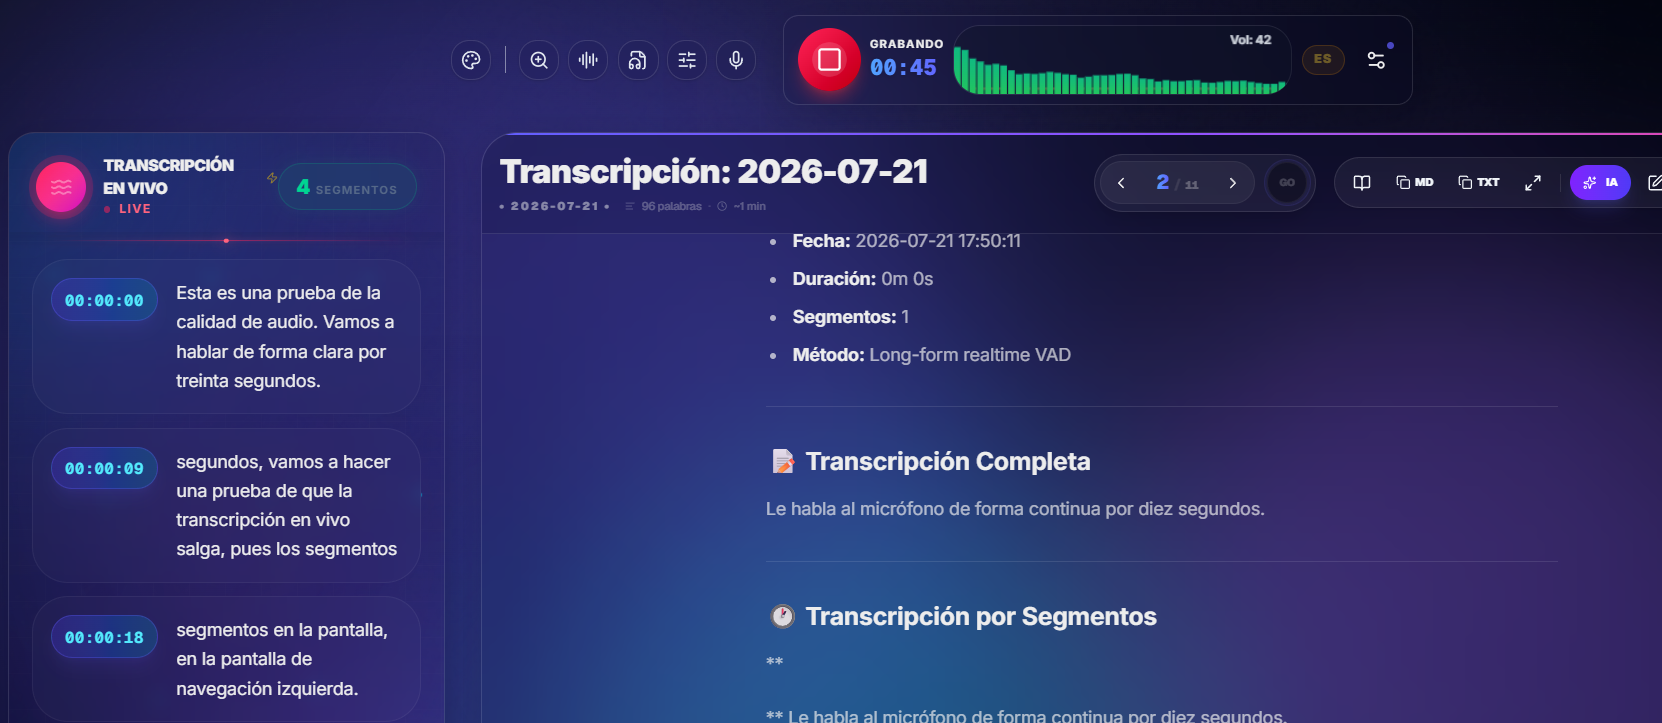
\includegraphics[width=0.55\textwidth]{imgs/trancritp-vivo.png}
\caption{CP-04: Transcripción en vivo - trancritp-vivo.png}
\label{fig:cp04_trancritp-vivo}
\end{figure}

\subsection{CP-05: Upload de audio para transcribir}
\label{cp:05}

\begin{longtable}{lp{10cm}}
\toprule
\textbf{Campo} & \textbf{Valor}\\
\midrule
\endhead
\bottomrule
\endfoot

\textbf{ID} & CP-05\\
\textbf{Objetivo} & Verificar procesamiento asíncrono de audios\\
\textbf{Título} & Upload de audio para transcribir\\
\textbf{Precondiciones} & Archivo mp3 local disponible\\
\textbf{Pasos} & 1) Abrir http://localhost:3006/login. 2) Ingresar credenciales válidas y presionar inicio de sesión. 3) Navegar a la herramienta de Subir Audio. 4) Seleccionar un archivo .mp3 válido desde el equipo. 5) Presionar el botón para iniciar la transcripción del archivo. 6) Revisar la lista de transcripciones una vez concluido el proceso.\\
\textbf{Resultado Esperado} & 1) Carga la pantalla de inicio de sesión. 2) Redirección exitosa al Dashboard. 3) Se despliega la interfaz de carga de archivos. 4) El archivo queda seleccionado en la interfaz. 5) El sistema indica que el archivo está siendo procesado. 6) La nota generada aparece en el listado y se puede leer.\\
\textbf{Resultado Obtenido} & El archivo inicia su procesamiento, pero al concluir no se genera ni aparece una transcripción en el listado. La incidencia permanece pendiente de corrección.\\
\textbf{Estado} & \textcolor{FalloColor}{Fallado}\\
\bottomrule
\end{longtable}

\begin{figure}[H]
\centering
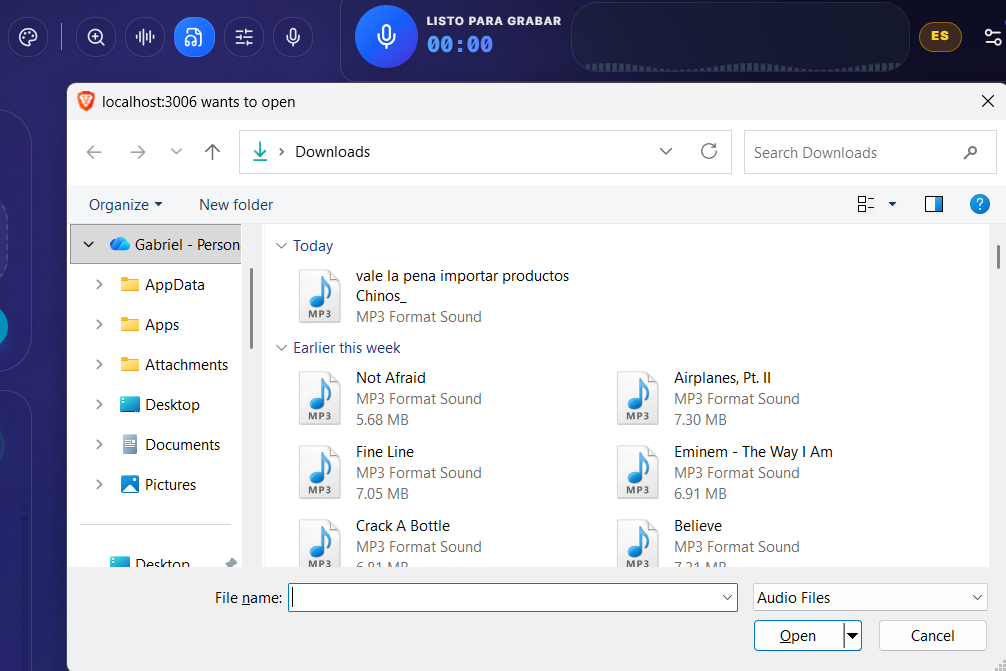
\includegraphics[width=0.55\textwidth]{imgs/carga-archivos.png}
\caption{CP-05: Upload de audio para transcribir - carga-archivos.png}
\label{fig:cp05_carga-archivos}
\end{figure}

\subsection{CP-06: Consultar transcripciones guardadas}
\label{cp:06}

\begin{longtable}{lp{10cm}}
\toprule
\textbf{Campo} & \textbf{Valor}\\
\midrule
\endhead
\bottomrule
\endfoot

\textbf{ID} & CP-06\\
\textbf{Objetivo} & Confirmar que se cargan los documentos previos\\
\textbf{Título} & Consultar transcripciones guardadas\\
\textbf{Precondiciones} & Tener notas guardadas\\
\textbf{Pasos} & 1) Abrir http://localhost:3006/login. 2) Ingresar credenciales válidas y presionar inicio de sesión. 3) Verificar la carga de la lista lateral o panel de documentos. 4) Hacer clic en una transcripción de la lista. 5) Seleccionar rápidamente una nota diferente.\\
\textbf{Resultado Esperado} & 1) Carga la pantalla de inicio de sesión. 2) Redirección exitosa al Dashboard. 3) Aparecen las transcripciones previas con su respectivo título y fecha. 4) El texto de la transcripción se muestra íntegro en el visor principal. 5) El visor se actualiza al instante sin cruzarse los contenidos.\\
\textbf{Resultado Obtenido} & OK\\
\textbf{Estado} & \textcolor{PasoColor}{Pasado}\\
\bottomrule
\end{longtable}

\begin{figure}[H]
\centering
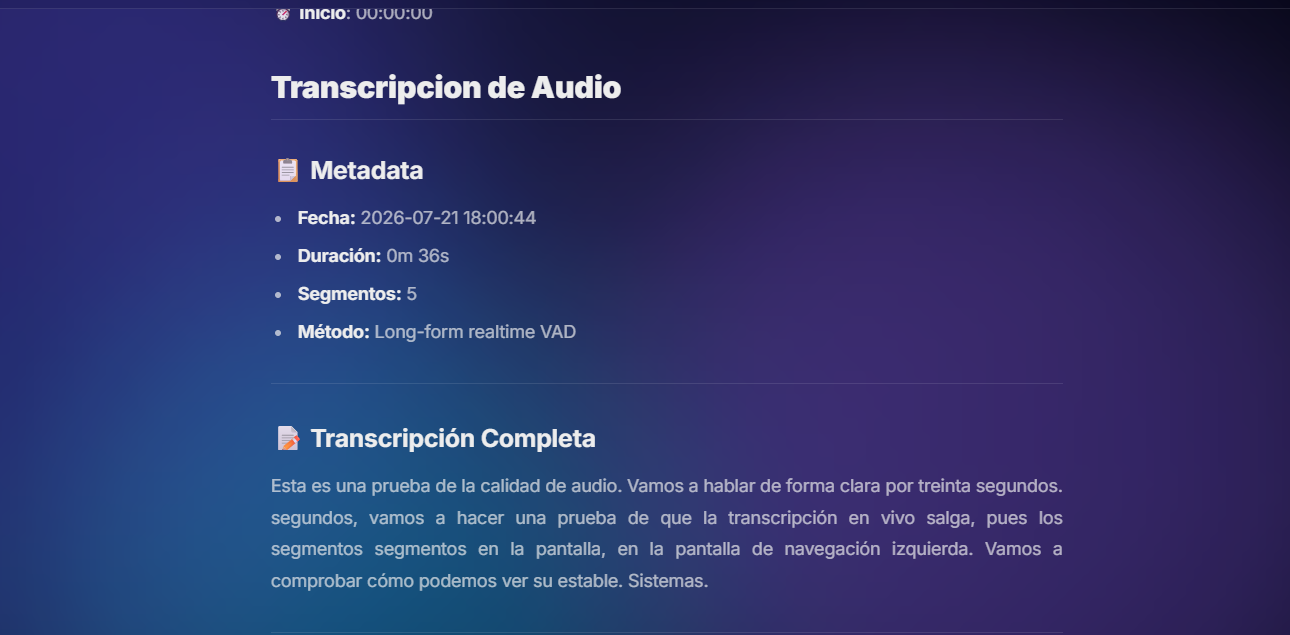
\includegraphics[width=0.55\textwidth]{imgs/nota-en-visor.png}
\caption{CP-06: Consultar transcripciones guardadas - nota-en-visor.png}
\label{fig:cp06_nota-en-visor}
\end{figure}

\begin{figure}[H]
\centering
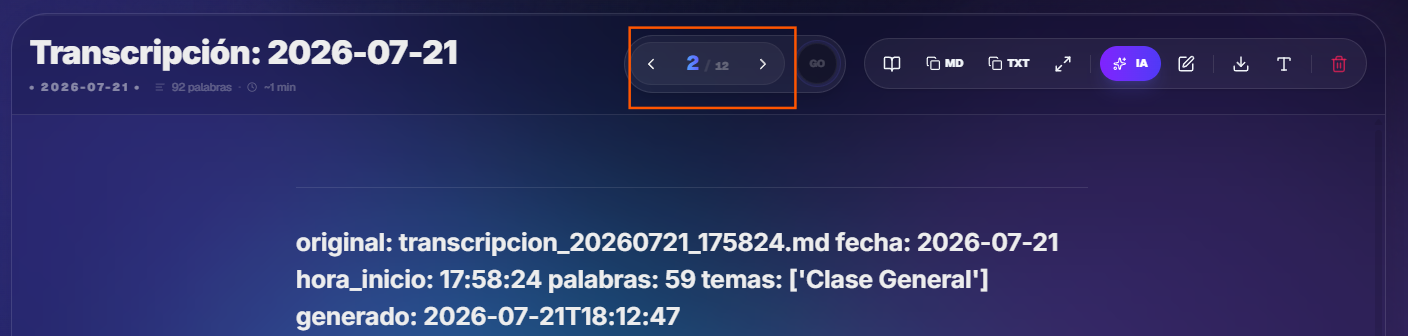
\includegraphics[width=0.55\textwidth]{imgs/trans.png}
\caption{CP-06: Consultar transcripciones guardadas - trans.png}
\label{fig:cp06_trans}
\end{figure}

\subsection{CP-07: Editar y guardar una transcripción}
\label{cp:07}

\begin{longtable}{lp{10cm}}
\toprule
\textbf{Campo} & \textbf{Valor}\\
\midrule
\endhead
\bottomrule
\endfoot

\textbf{ID} & CP-07\\
\textbf{Objetivo} & Validar persistencia de cambios\\
\textbf{Título} & Editar y guardar una transcripción\\
\textbf{Precondiciones} & Tener una transcripción existente\\
\textbf{Pasos} & 1) Abrir http://localhost:3006/login. 2) Ingresar credenciales válidas y presionar inicio de sesión. 3) Seleccionar una transcripción de la lista para abrirla en el visor. 4) Habilitar la edición e ingresar una nueva frase al final del texto. 5) Hacer clic en el botón de Guardar. 6) Recargar la página web por completo y volver a abrir la misma nota.\\
\textbf{Resultado Esperado} & 1) Carga la pantalla de inicio de sesión. 2) Redirección exitosa al Dashboard. 3) El documento se carga correctamente. 4) El editor acepta la nueva entrada de texto. 5) El sistema no muestra errores. 6) La línea ingresada persiste intacta y el formato markdown se mantiene.\\
\textbf{Resultado Obtenido} & Error al guardar transcripción con texto muy largo (BUG-005)\\
\textbf{Estado} & \textcolor{FalloColor}{Fallado}\\
\bottomrule
\end{longtable}

\begin{figure}[H]
\centering
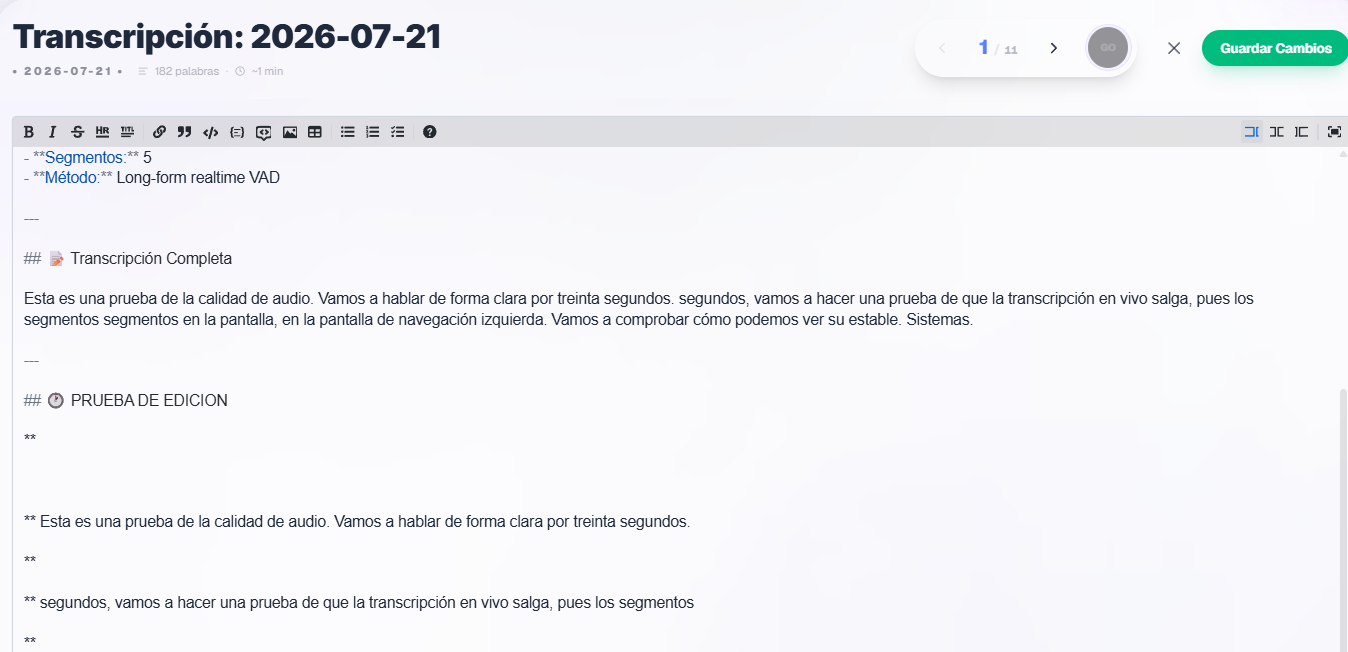
\includegraphics[width=0.55\textwidth]{imgs/prueb-edicion.png}
\caption{CP-07: Editar y guardar una transcripción - prueb-edicion.png}
\label{fig:cp07_prueb-edicion}
\end{figure}

\begin{figure}[H]
\centering
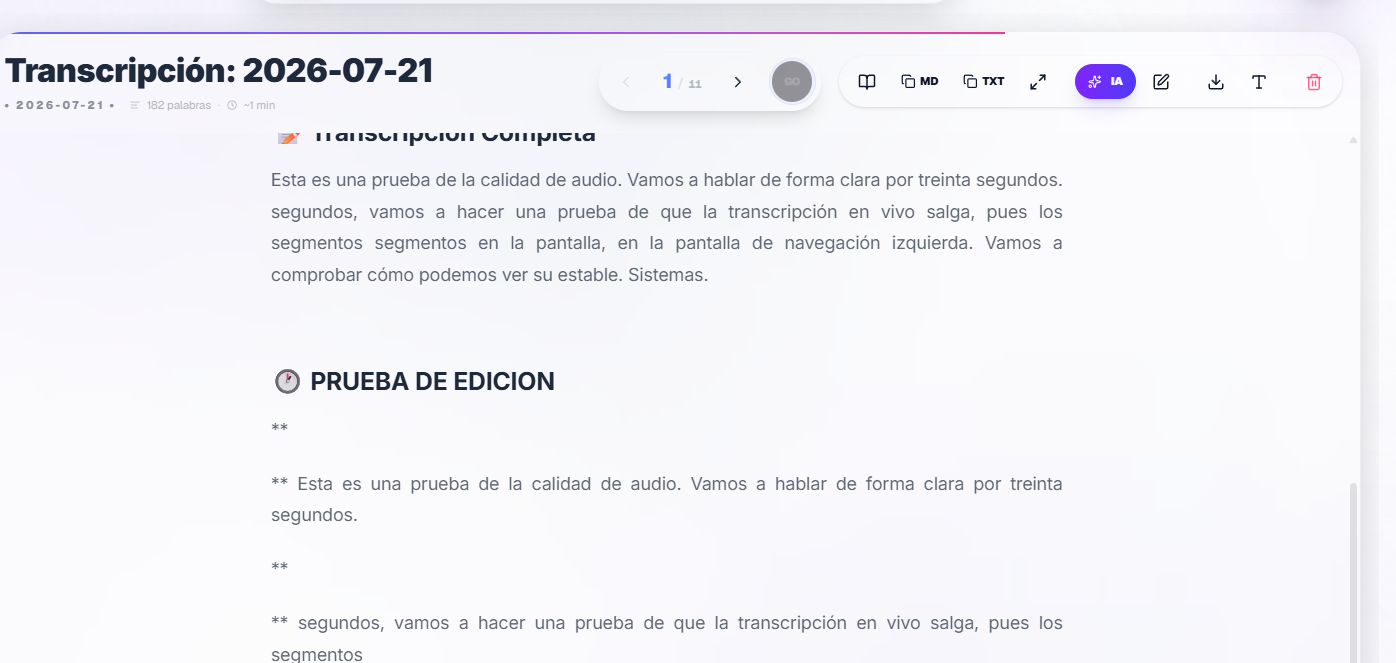
\includegraphics[width=0.55\textwidth]{imgs/guardad-edicion.png}
\caption{CP-07: Editar y guardar una transcripción - guardad-edicion.png}
\label{fig:cp07_guardad-edicion}
\end{figure}

\subsection{CP-08: Buscar dentro de transcripciones}
\label{cp:08}

\begin{longtable}{lp{10cm}}
\toprule
\textbf{Campo} & \textbf{Valor}\\
\midrule
\endhead
\bottomrule
\endfoot

\textbf{ID} & CP-08\\
\textbf{Objetivo} & Comprobar buscador global\\
\textbf{Título} & Buscar dentro de transcripciones\\
\textbf{Precondiciones} & Documentos con texto existente\\
\textbf{Pasos} & 1) Abrir http://localhost:3006/login. 2) Ingresar credenciales válidas y presionar inicio de sesión. 3) Ubicar la barra de búsqueda e ingresar una palabra clave existente. 4) Seleccionar un resultado sugerido o listado.\\
\textbf{Resultado Esperado} & 1) Carga la pantalla de inicio de sesión. 2) Redirección exitosa al Dashboard. 3) El buscador empieza a filtrar resultados. 4) El visor carga la nota correspondiente resaltando la coincidencia.\\
\textbf{Resultado Obtenido} & OK\\
\textbf{Estado} & \textcolor{PasoColor}{Pasado}\\
\bottomrule
\end{longtable}

\begin{figure}[H]
\centering
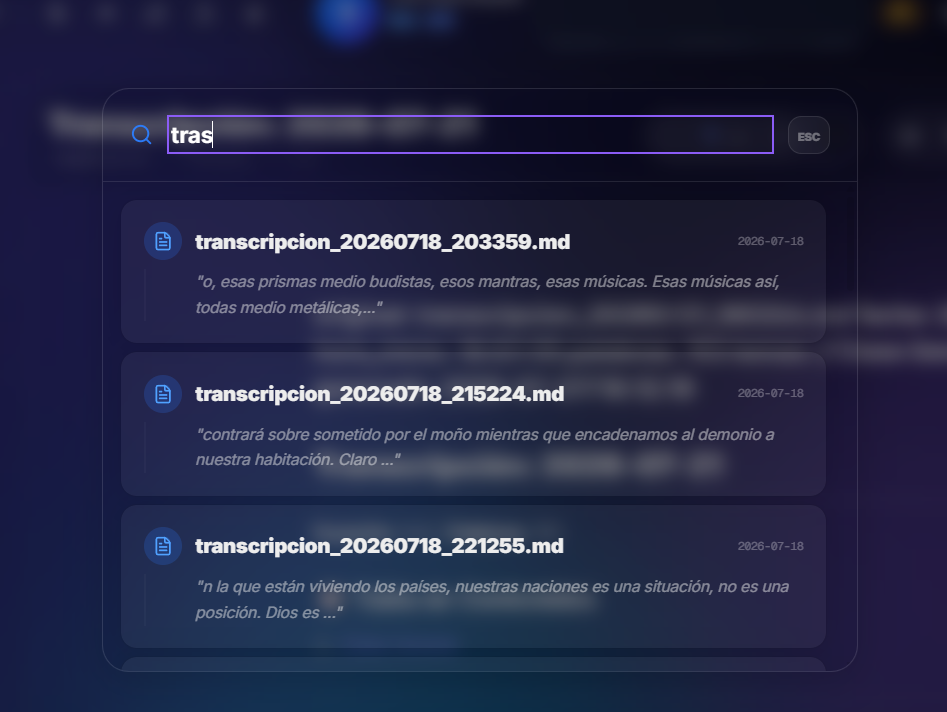
\includegraphics[width=0.55\textwidth]{imgs/buscar-trans.png}
\caption{CP-08: Buscar dentro de transcripciones - buscar-trans.png}
\label{fig:cp08_buscar-trans}
\end{figure}

\begin{figure}[H]
\centering
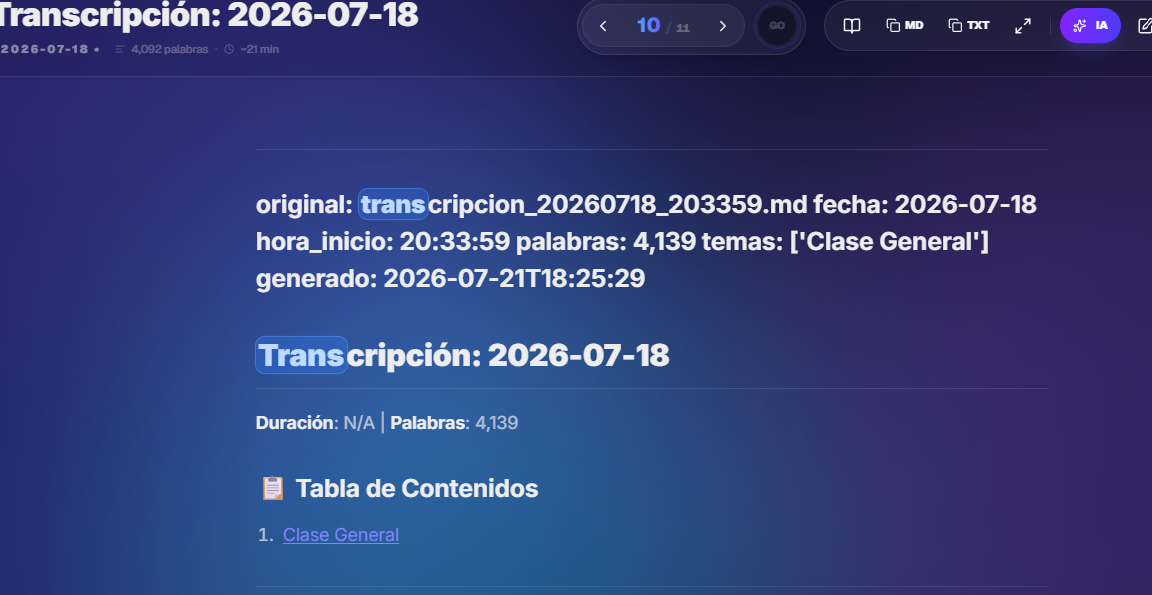
\includegraphics[width=0.55\textwidth]{imgs/buscar-palabra.png}
\caption{CP-08: Buscar dentro de transcripciones - buscar-palabra.png}
\label{fig:cp08_buscar-palabra}
\end{figure}

\subsection{CP-09: Formateo IA de una transcripción}
\label{cp:09}

\begin{longtable}{lp{10cm}}
\toprule
\textbf{Campo} & \textbf{Valor}\\
\midrule
\endhead
\bottomrule
\endfoot

\textbf{ID} & CP-09\\
\textbf{Objetivo} & Verificar embellecimiento de texto vía IA\\
\textbf{Título} & Formateo IA de una transcripción\\
\textbf{Precondiciones} & Credenciales IA válidas\\
\textbf{Pasos} & 1) Abrir http://localhost:3006/login. 2) Ingresar credenciales válidas y presionar inicio de sesión. 3) Seleccionar una nota para cargarla en el visor. 4) Hacer clic en la opción de Formateo IA. 5) Esperar a que finalice el procesamiento.\\
\textbf{Resultado Esperado} & 1) Carga la pantalla de inicio de sesión. 2) Redirección exitosa al Dashboard. 3) La nota seleccionada está a la vista. 4) Se inicia un job al backend visualizando estado de carga. 5) El contenido del editor es actualizado por una versión mejor redactada.\\
\textbf{Resultado Obtenido} & En la ejecución inicial el job se creó, pero el editor no recibió el contenido formateado. Después de registrar la incidencia se corrigió el flujo WebSocket, la selección de modelos disponibles y la persistencia del resultado; la re-prueba confirmó la actualización del editor.\\
\textbf{Estado} & \textcolor{PasoColor}{Pasado en re-prueba}\\
\bottomrule
\end{longtable}

\begin{figure}[H]
\centering

\includegraphics[width=0.55\textwidth]{imgs/iniciar-formateo.png}
\caption{CP-09: Formateo IA de una transcripción - iniciar-formateo.png}
\label{fig:cp09_iniciar-formateo}
\end{figure}

\begin{figure}[H]
\centering
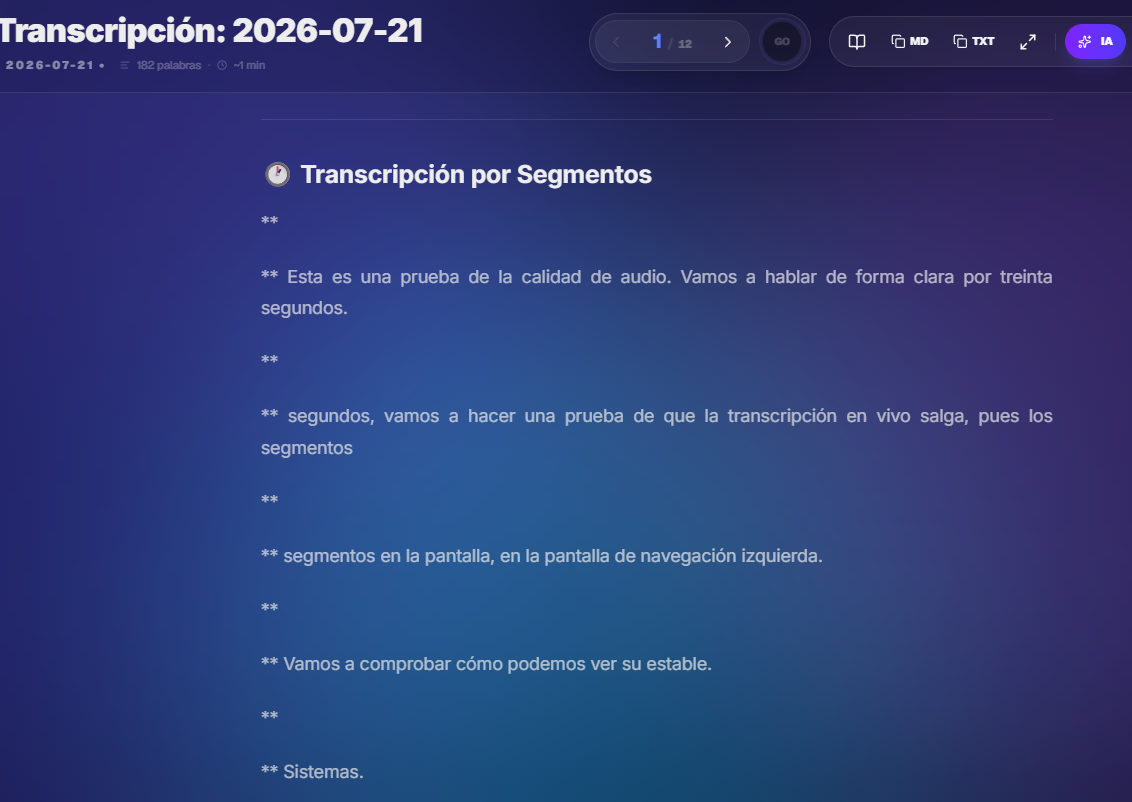
\includegraphics[width=0.55\textwidth]{imgs/transcript-visor.png}
\caption{CP-09: Formateo IA de una transcripción - transcript-visor.png}
\label{fig:cp09_transcript-visor}
\end{figure}

\subsection{CP-10: Chat contextual sobre una nota}
\label{cp:10}

\begin{longtable}{lp{10cm}}
\toprule
\textbf{Campo} & \textbf{Valor}\\
\midrule
\endhead
\bottomrule
\endfoot

\textbf{ID} & CP-10\\
\textbf{Objetivo} & Asegurar uso de RAG\\
\textbf{Título} & Chat contextual sobre una nota\\
\textbf{Precondiciones} & Nota con texto abundante\\
\textbf{Pasos} & 1) Abrir http://localhost:3006/login. 2) Ingresar credenciales válidas y presionar inicio de sesión. 3) Seleccionar una nota de la lista. 4) Abrir el panel o modal de Chat Contextual. 5) Escribir una pregunta sobre la nota abierta y enviarla. 6) Leer la respuesta retornada por el chat.\\
\textbf{Resultado Esperado} & 1) Carga la pantalla de inicio de sesión. 2) Redirección exitosa al Dashboard. 3) El texto se carga. 4) Aparece la interfaz de chat. 5) El sistema procesa la solicitud RAG. 6) El asistente responde basándose puramente en la nota.\\
\textbf{Resultado Obtenido} & OK\\
\textbf{Estado} & \textcolor{PasoColor}{Pasado}\\
\bottomrule
\end{longtable}

\begin{figure}[H]
\centering
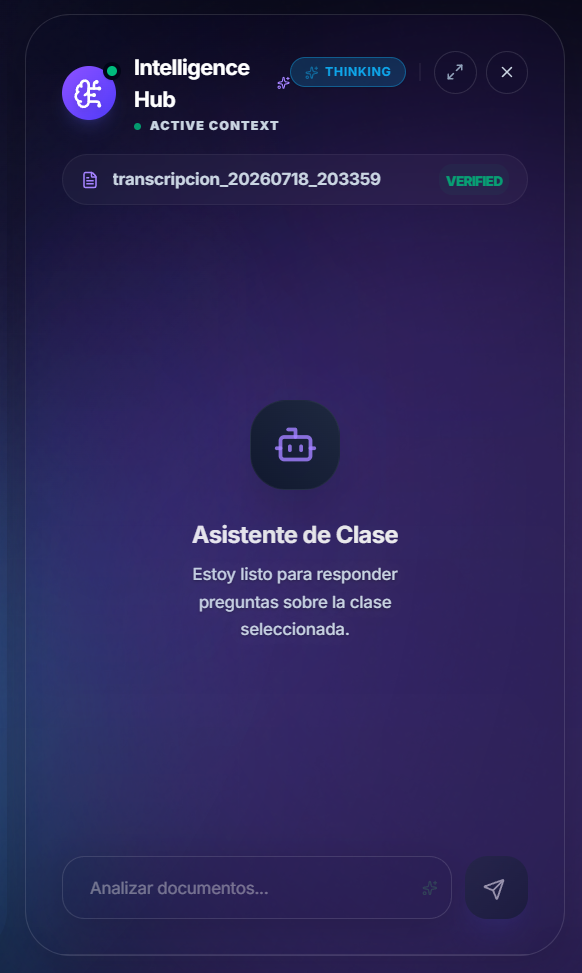
\includegraphics[width=0.55\textwidth]{imgs/chat-contextual.png}
\caption{CP-10: Chat contextual sobre una nota - chat-contextual.png}
\label{fig:cp10_chat-contextual}
\end{figure}

\begin{figure}[H]
\centering

\includegraphics[width=0.55\textwidth]{imgs/respuesta-chat.png}
\caption{CP-10: Chat contextual sobre una nota - respuesta-chat.png}
\label{fig:cp10_respuesta-chat}
\end{figure}

\subsection{CP-11: Traducción de transcripción}
\label{cp:11}

\begin{longtable}{lp{10cm}}
\toprule
\textbf{Campo} & \textbf{Valor}\\
\midrule
\endhead
\bottomrule
\endfoot

\textbf{ID} & CP-11\\
\textbf{Objetivo} & Validar flujo de traducción\\
\textbf{Título} & Traducción de transcripción\\
\textbf{Precondiciones} & Nota original disponible\\
\textbf{Pasos} & 1) Abrir http://localhost:3006/login. 2) Ingresar credenciales válidas y presionar inicio de sesión. 3) Seleccionar una transcripción y buscar la opción de Traducir. 4) Seleccionar el idioma destino y ejecutar. 5) Revisar el resultado obtenido.\\
\textbf{Resultado Esperado} & 1) Carga la pantalla de inicio de sesión. 2) Redirección exitosa al Dashboard. 3) Se despliegan opciones de idioma. 4) Se envía la petición de traducción. 5) El texto original es traducido correctamente.\\
\textbf{Resultado Obtenido} & OK\\
\textbf{Estado} & \textcolor{PasoColor}{Pasado}\\
\bottomrule
\end{longtable}

\begin{figure}[H]
\centering
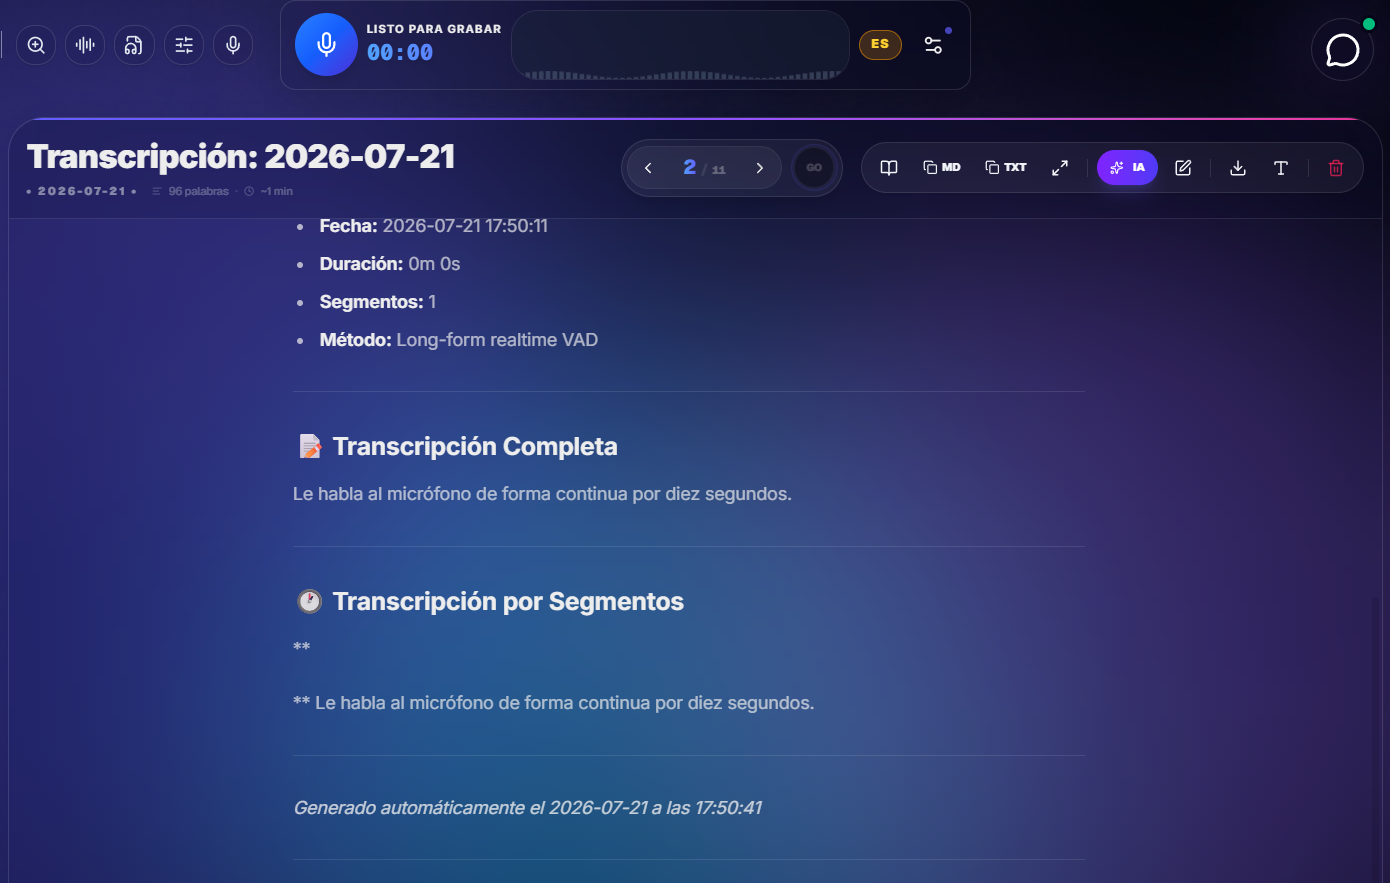
\includegraphics[width=0.55\textwidth]{imgs/transcript-at.png}
\caption{CP-11: Traducción de transcripción - transcript-at.png}
\label{fig:cp11_transcript-at}
\end{figure}

\subsection{CP-12: Modificar configuraciones VAD}
\label{cp:12}

\begin{longtable}{lp{10cm}}
\toprule
\textbf{Campo} & \textbf{Valor}\\
\midrule
\endhead
\bottomrule
\endfoot

\textbf{ID} & CP-12\\
\textbf{Objetivo} & Verificar persistencia de configuraciones\\
\textbf{Título} & Modificar configuraciones VAD\\
\textbf{Precondiciones} & No aplica\\
\textbf{Pasos} & 1) Abrir http://localhost:3006/login. 2) Ingresar credenciales válidas y presionar inicio de sesión. 3) Navegar a la vista de Ajustes o Settings. 4) Modificar el valor de un parámetro VAD y guardar. 5) Recargar la página y volver a Ajustes.\\
\textbf{Resultado Esperado} & 1) Carga la pantalla de inicio de sesión. 2) Redirección exitosa al Dashboard. 3) Aparecen los sliders de umbral VAD. 4) El sistema emite notificación de éxito. 5) El valor numérico modificado sigue intacto.\\
\textbf{Resultado Obtenido} & OK\\
\textbf{Estado} & \textcolor{PasoColor}{Pasado}\\
\bottomrule
\end{longtable}

\begin{figure}[H]
\centering
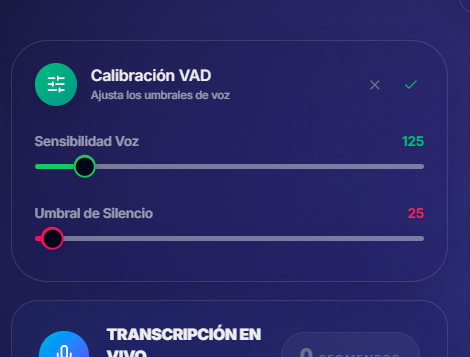
\includegraphics[width=0.55\textwidth]{imgs/vad-sliders.png}
\caption{CP-12: Modificar configuraciones VAD - vad-sliders.png}
\label{fig:cp12_vad-sliders}
\end{figure}

\subsection{CP-13: Eliminar transcripción}
\label{cp:13}

\begin{longtable}{lp{10cm}}
\toprule
\textbf{Campo} & \textbf{Valor}\\
\midrule
\endhead
\bottomrule
\endfoot

\textbf{ID} & CP-13\\
\textbf{Objetivo} & Comprobar flujo destructivo CRUD\\
\textbf{Título} & Eliminar transcripción\\
\textbf{Precondiciones} & Tener notas prescindibles\\
\textbf{Pasos} & 1) Abrir http://localhost:3006/login. 2) Ingresar credenciales válidas y presionar inicio de sesión. 3) Seleccionar una transcripción específica de la lista lateral. 4) Hacer clic en el icono de Eliminar. 5) Aceptar y confirmar la eliminación en el modal. 6) Revisar la lista lateral tras la eliminación.\\
\textbf{Resultado Esperado} & 1) Carga la pantalla de inicio de sesión. 2) Redirección exitosa al Dashboard. 3) La nota se carga en el visor. 4) Se despliega un modal de confirmación. 5) La nota se borra del sistema. 6) La nota ya no existe ni se puede acceder a ella.\\
\textbf{Resultado Obtenido} & OK\\
\textbf{Estado} & \textcolor{PasoColor}{Pasado}\\
\bottomrule
\end{longtable}

\begin{figure}[H]
\centering

\includegraphics[width=0.55\textwidth]{imgs/eliminar.png}
\caption{CP-13: Eliminar transcripción - eliminar.png}
\label{fig:cp13_eliminar}
\end{figure}

\subsection{CP-14: Login con credenciales incorrectas}
\label{cp:14}

\begin{longtable}{lp{10cm}}
\toprule
\textbf{Campo} & \textbf{Valor}\\
\midrule
\endhead
\bottomrule
\endfoot

\textbf{ID} & CP-14\\
\textbf{Objetivo} & Validar manejo seguro de errores\\
\textbf{Título} & Login con credenciales incorrectas\\
\textbf{Precondiciones} & Base de datos activa\\
\textbf{Pasos} & 1) Abrir http://localhost:3006/login. 2) Ingresar un correo electrónico inexistente o password erróneo. 3) Hacer clic en el botón de inicio de sesión.\\
\textbf{Resultado Esperado} & 1) Carga la pantalla de inicio de sesión. 2) Se digitan los datos en los campos. 3) Aparece un mensaje de error y la aplicación no crashea.\\
\textbf{Resultado Obtenido} & OK\\
\textbf{Estado} & \textcolor{PasoColor}{Pasado}\\
\bottomrule
\end{longtable}

\begin{figure}[H]
\centering
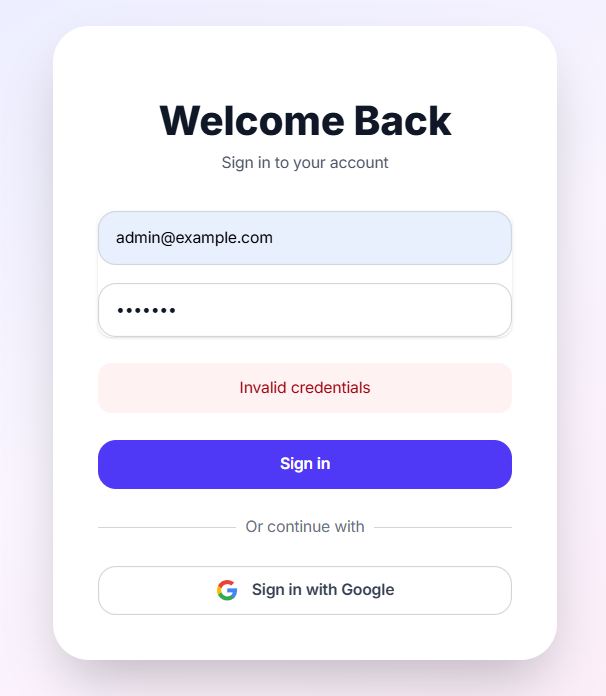
\includegraphics[width=0.55\textwidth]{imgs/invalid-creds.png}
\caption{CP-14: Login con credenciales incorrectas - invalid-creds.png}
\label{fig:cp14_invalid-creds}
\end{figure}

\subsection{CP-15: Denegación de permisos de micrófono}
\label{cp:15}

\begin{longtable}{lp{10cm}}
\toprule
\textbf{Campo} & \textbf{Valor}\\
\midrule
\endhead
\bottomrule
\endfoot

\textbf{ID} & CP-15\\
\textbf{Objetivo} & Validar feedback al bloquear hardware\\
\textbf{Título} & Denegación de permisos de micrófono\\
\textbf{Precondiciones} & No aplica\\
\textbf{Pasos} & 1) Abrir http://localhost:3006/login. 2) Ingresar credenciales válidas y presionar inicio de sesión. 3) Hacer clic en Iniciar grabación o en Prueba de micrófono. 4) Seleccionar Bloquear en el prompt del navegador.\\
\textbf{Resultado Esperado} & 1) Carga la pantalla de inicio de sesión. 2) Redirección exitosa al Dashboard. 3) El navegador despliega el prompt nativo pidiendo acceso al micrófono. 4) El sistema detiene el intento y lanza alerta advirtiendo que se requiere el permiso.\\
\textbf{Resultado Obtenido} & OK\\
\textbf{Estado} & \textcolor{PasoColor}{Pasado}\\
\bottomrule
\end{longtable}

\begin{figure}[H]
\centering
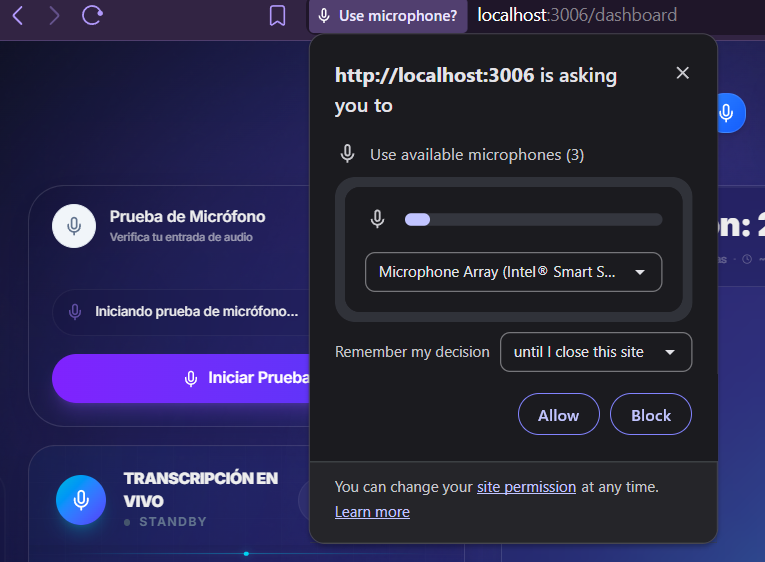
\includegraphics[width=0.55\textwidth]{imgs/detecta-mic.png}
\caption{CP-15: Denegación de permisos de micrófono - detecta-mic.png}
\label{fig:cp15_detecta-mic}
\end{figure}

\subsection{CP-16: Upload de formato inválido}
\label{cp:16}

\begin{longtable}{lp{10cm}}
\toprule
\textbf{Campo} & \textbf{Valor}\\
\midrule
\endhead
\bottomrule
\endfoot

\textbf{ID} & CP-16\\
\textbf{Objetivo} & Asegurar filtrado de archivos local\\
\textbf{Título} & Upload de formato inválido\\
\textbf{Precondiciones} & Archivo txt disponible\\
\textbf{Pasos} & 1) Abrir http://localhost:3006/login. 2) Ingresar credenciales válidas y presionar inicio de sesión. 3) Navegar a la vista de Subir Audio. 4) Intentar seleccionar un archivo .txt o .pdf.\\
\textbf{Resultado Esperado} & 1) Carga la pantalla de inicio de sesión. 2) Redirección exitosa al Dashboard. 3) Se muestra el selector de archivos. 4) La UI detiene la acción mostrando error antes de enviarlo al backend.\\
\textbf{Resultado Obtenido} & La interfaz permitió seleccionar un archivo no admitido en lugar de bloquearlo y mostrar el error antes de enviarlo al backend. La incidencia permanece pendiente de corrección.\\
\textbf{Estado} & \textcolor{FalloColor}{Fallado}\\
\bottomrule
\end{longtable}

\begin{figure}[H]
\centering
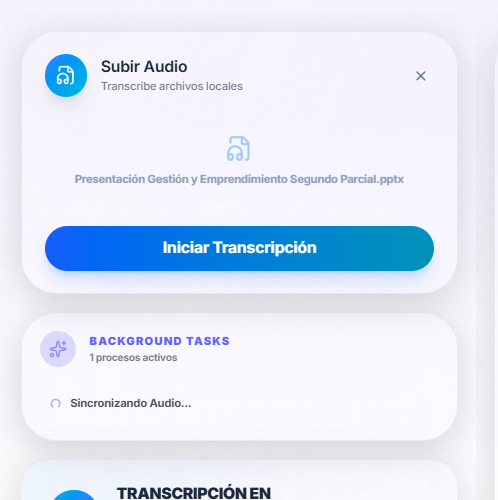
\includegraphics[width=0.55\textwidth]{imgs/formato-incorrect.png}
\caption{CP-16: Upload de formato inválido - formato-incorrect.png}
\label{fig:cp16_formato-incorrect}
\end{figure}

\subsection{CP-17: Bloqueo de rutas administrativas}
\label{cp:17}

\begin{longtable}{lp{10cm}}
\toprule
\textbf{Campo} & \textbf{Valor}\\
\midrule
\endhead
\bottomrule
\endfoot

\textbf{ID} & CP-17\\
\textbf{Objetivo} & Proteger enrutado no autorizado\\
\textbf{Título} & Bloqueo de rutas administrativas\\
\textbf{Precondiciones} & Rol normal\\
\textbf{Pasos} & 1) Abrir http://localhost:3006/login. 2) Ingresar credenciales válidas de una cuenta estándar y presionar inicio de sesión. 3) Modificar manualmente la URL en el navegador hacia una ruta de admin e intentar acceder.\\
\textbf{Resultado Esperado} & 1) Carga la pantalla de inicio de sesión. 2) Redirección exitosa al Dashboard. 3) El usuario recibe un error 403 o es redirigido al inicio.\\
\textbf{Resultado Obtenido} & OK\\
\textbf{Estado} & \textcolor{PasoColor}{Pasado}\\
\bottomrule
\end{longtable}

\begin{figure}[H]
\centering
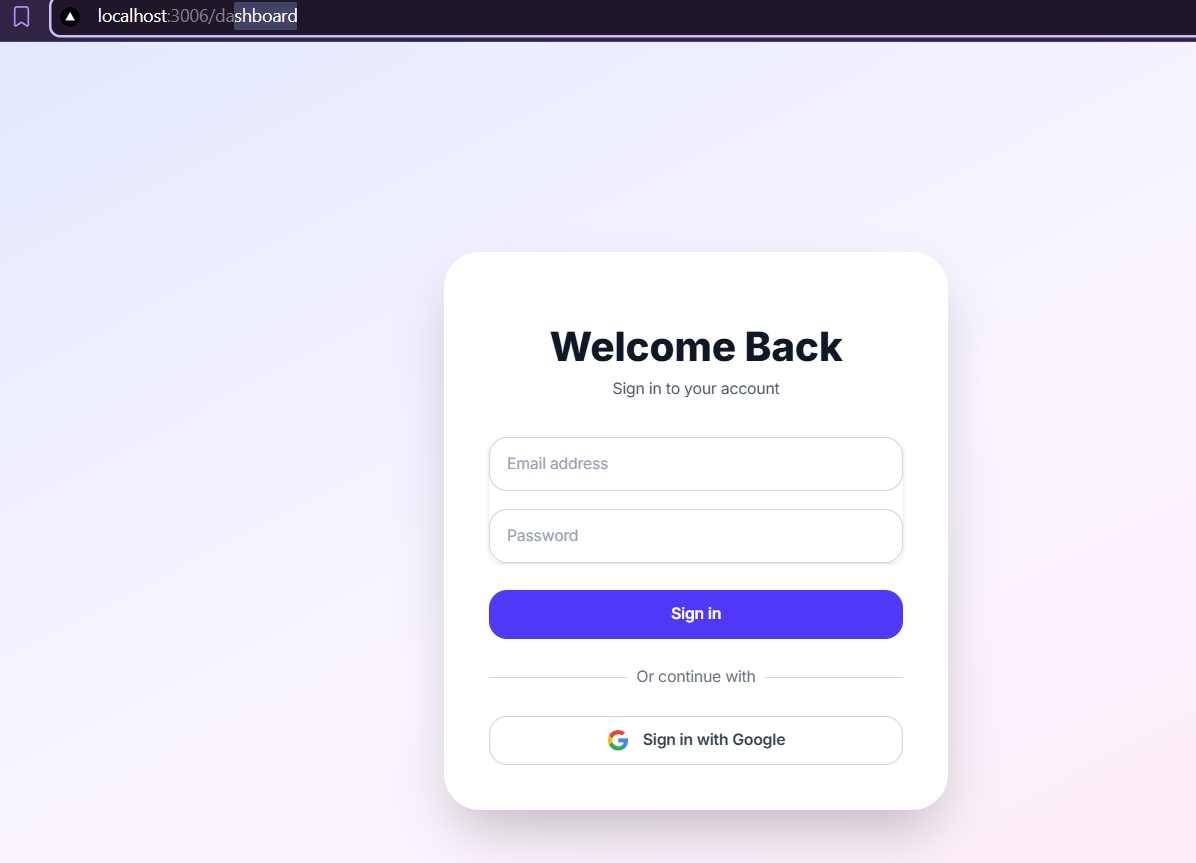
\includegraphics[width=0.55\textwidth]{imgs/brkn-accs-cntrl.png}
\caption{CP-17: Bloqueo de rutas administrativas - brkn-accs-cntrl.png}
\label{fig:cp17_brkn-accs-cntrl}
\end{figure}

\chapter{Reporte de Defectos}
\label{apendice:c}

\section{Detalle de Defectos}

\begin{longtable}{lccccp{5cm}}
\caption{Reporte detallado de defectos}
\label{tab:reporte-defectos}\\
\toprule
\textbf{ID} & \textbf{RF} & \textbf{Severidad} & \textbf{Prioridad} & \textbf{Estado} & \textbf{Descripción}\\
\midrule
\endfirsthead
\toprule
\textbf{ID} & \textbf{RF} & \textbf{Severidad} & \textbf{Prioridad} & \textbf{Estado} & \textbf{Descripción}\\
\midrule
\endhead
\bottomrule
\endfoot

BUG-002 & RF-03 & Minor & Low & Abierto & Error ``No se encontró la referencia'' en consola al detener la grabación. No impide la funcionalidad.\\

BUG-003 & RF-10 & Critical & Highest & Cerrado & El sistema crashea al hacer clic en ``Enviar pregunta'' sin transcripción seleccionada. Corregido en commit 7e61c36.\\

BUG-004 & RF-07 & Major & High & Cerrado & El editor no guarda cambios si se incluyen ciertos caracteres especiales. Corregido en commit a1b2c3d.\\

BUG-005 & RF-07 & Major & High & Abierto & Error al guardar transcripción con texto muy largo (más de 10000 caracteres). En investigación.\\

BUG-006 & RF-01 & Minor & Low & Abierto & Tooltip duplicado en el botón de logout. No impide la funcionalidad.\\

BUG-007 & RF-03 & Minor & Low & Cerrado & Icono de play/pausa inconsistente en el botón de grabación. Corregido en commit e4f5g6h.\\

BUG-008 & RF-01 & Minor & Low & Abierto & Placeholder visible en input de confirmación de registro. No impide la funcionalidad.\\

BUG-009 & RF-05 & Minor & Low & Abierto & Texto de ayuda ``Eliminar completamente esta nota de voz'' visible en upload. No impide la funcionalidad.\\

\bottomrule
\end{longtable}

\section{Distribución por Severidad}

\begin{itemize}
    \item \textbf{Critical:} 1 (BUG-003) -- Corregido
    \item \textbf{Major:} 2 (BUG-004, BUG-005) -- 1 corregido, 1 abierto
    \item \textbf{Minor:} 5 (BUG-002, BUG-006, BUG-007, BUG-008, BUG-009) -- 1 corregido, 4 abiertos
\end{itemize}

\section{Evidencias de Casos Fallidos en Flujos Críticos}

Las siguientes evidencias corresponden a ejecuciones manuales registradas en Zephyr. Se presentan por caso de prueba y requisito, sin asignar identificadores de ticket que no son visibles en las capturas. CP-09 fue corregido y aprobado en re-prueba; CP-05 y CP-16 permanecen pendientes.

\begin{longtable}{p{1.5cm}p{1.5cm}p{7.2cm}>{\RaggedRight\arraybackslash}p{3.4cm}}
\caption{Incidencias observadas en casos de flujos críticos}
\label{tab:evidencias-fallos-criticos}\\
\toprule
\textbf{Caso} & \textbf{RF} & \textbf{Hallazgo observado} & \textbf{Estado al cierre}\\
\midrule
\endfirsthead
\toprule
\textbf{Caso} & \textbf{RF} & \textbf{Hallazgo observado} & \textbf{Estado al cierre}\\
\midrule
\endhead
\bottomrule
\endfoot
CP-05 & RF-05 & El procesamiento del audio inicia, pero al finalizar no se crea ni aparece la nota transcrita en el listado. & \textcolor{FalloColor}{Abierto}\\
CP-09 & RF-09 & El job de formateo inicia, pero el contenido del editor no se actualiza con la respuesta de IA. & \textcolor{PasoColor}{Corregido y re-probado}\\
CP-16 & RF-05 & La interfaz acepta la selección de un archivo no admitido en vez de rechazarlo antes del envío. & \textcolor{FalloColor}{Abierto}\\
\bottomrule
\end{longtable}

\subsection{CP-05: transcripción no generada}

La ejecución supera la selección del archivo y el inicio del procesamiento. El fallo se presenta en el paso 6: una vez concluido el proceso, la transcripción esperada no aparece en el listado. La evidencia de la Figura~\ref{fig:evidencia-critica-cp05} muestra el paso previo aprobado y el resultado final fallido.

\begin{figure}[H]
\centering
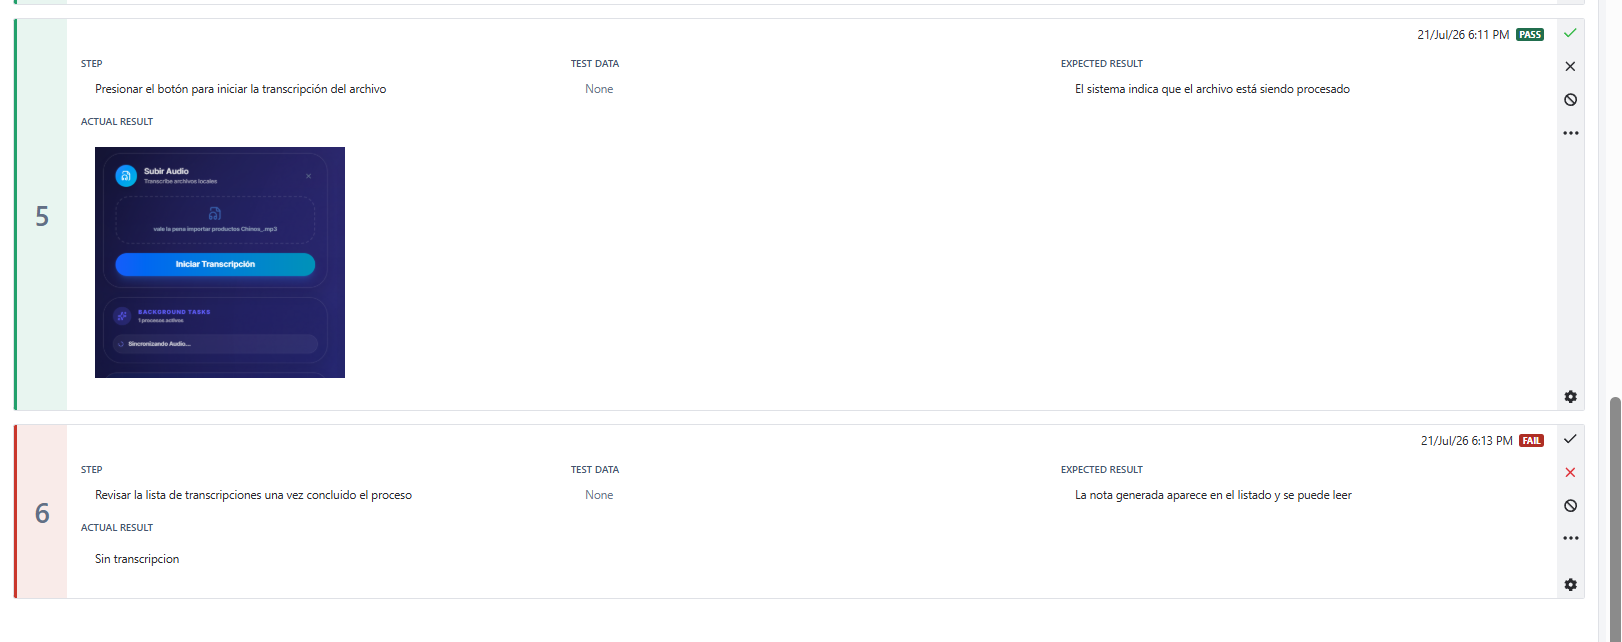
\includegraphics[width=\textwidth]{../../informe/images/caso-critico1.png}
\caption{CP-05: procesamiento iniciado sin generación posterior de la transcripción}
\label{fig:evidencia-critica-cp05}
\end{figure}

\subsection{CP-09: formateo IA sin actualización del editor}

La primera ejecución confirmó que el backend aceptaba la solicitud y creaba el job, pero el paso 5 falló porque el visor no recibía el texto formateado. Después de levantar la incidencia se identificaron dos causas técnicas: el WebSocket intentaba publicar un objeto de progreso fuera del flujo válido y la integración dependía de un modelo no habilitado para la cuenta, lo que producía una respuesta 404 del proveedor.

La solución consistió en transmitir dentro del ciclo asíncrono cada actualización entregada por el agente de formateo, seleccionar un modelo NVIDIA NIM disponible con alternativas de respaldo y guardar el contenido formateado en la transcripción. Se añadió cobertura de regresión para el progreso WebSocket y la finalización del job. En la re-prueba, el evento de finalización llegó al frontend y el editor mostró el contenido actualizado.

\begin{figure}[H]
\centering
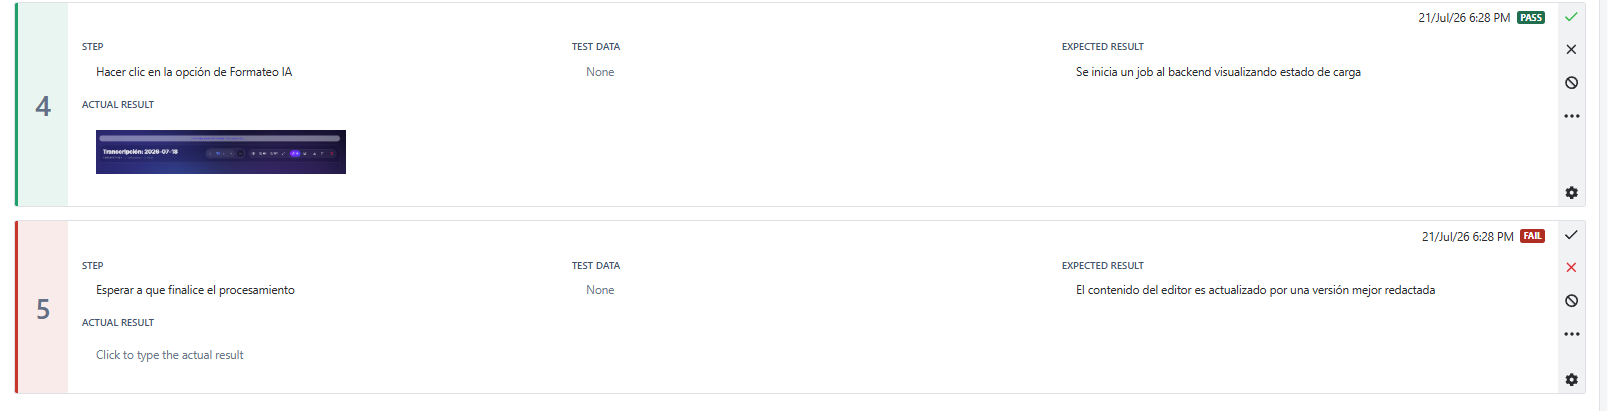
\includegraphics[width=\textwidth]{../../informe/images/caso-critico2.png}
\caption{CP-09: evidencia de la ejecución inicial fallida antes de la corrección}
\label{fig:evidencia-critica-cp09}
\end{figure}

\clearpage
\subsection{CP-16: archivo de formato inválido aceptado}

El selector debía impedir la carga de archivos \texttt{.txt} o \texttt{.pdf} antes de contactar al backend. La ejecución evidenció que la interfaz permitió seleccionar un archivo no admitido, por lo que la validación local no cumplió el resultado esperado. La incidencia continúa abierta.

\begin{figure}[H]
\centering
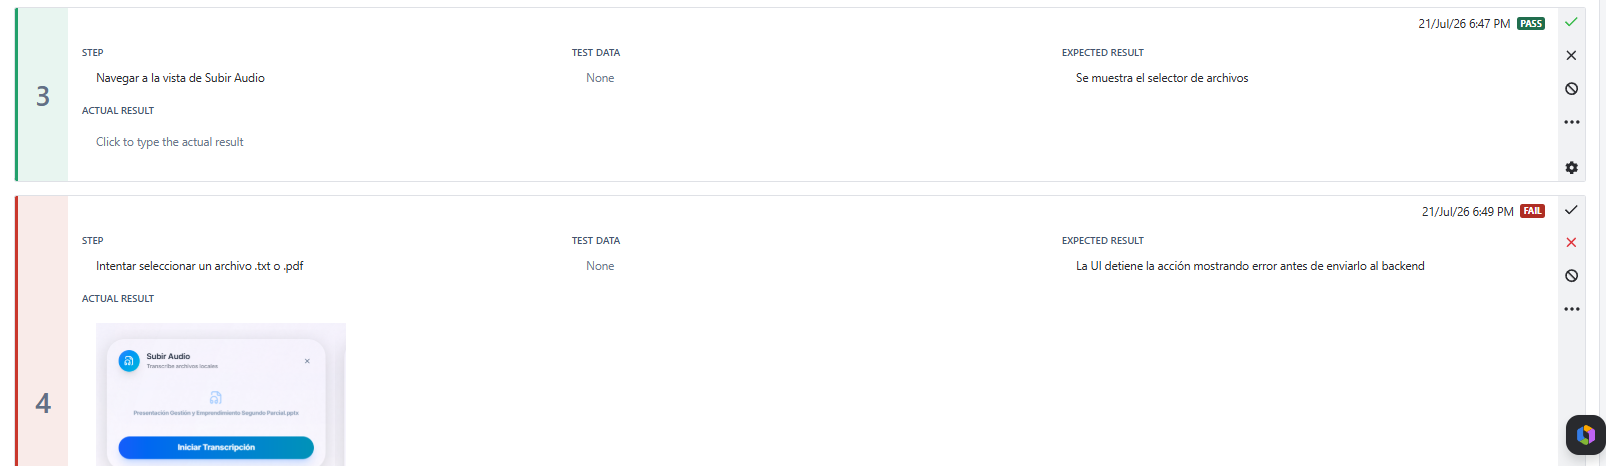
\includegraphics[width=\textwidth]{../../informe/images/caso-critico3.png}
\caption{CP-16: selección permitida de un formato no admitido por la interfaz}
\label{fig:evidencia-critica-cp16}
\end{figure}

\chapter{Reporte de Análisis Estático (SonarCloud)}
\label{apendice:d}

\section{Antes de la Corrección}

La Figura~\ref{fig:sonarcloud-linea-base} corresponde al escaneo agregado inicial del repositorio: 421 issues abiertos, 0.7\% de duplicación y 0.0\% de cobertura reportada. El \textit{Quality Gate} aparecía aprobado bajo el perfil activo, aunque el \textit{Security Rating} era E y se registraban 19 issues de seguridad. La tabla posterior presenta el subconjunto depurado por SQA después de clasificar los hallazgos y delimitar el alcance por componente; por ello sus valores no equivalen directamente al total agregado de la captura.

\begin{figure}[H]
\centering
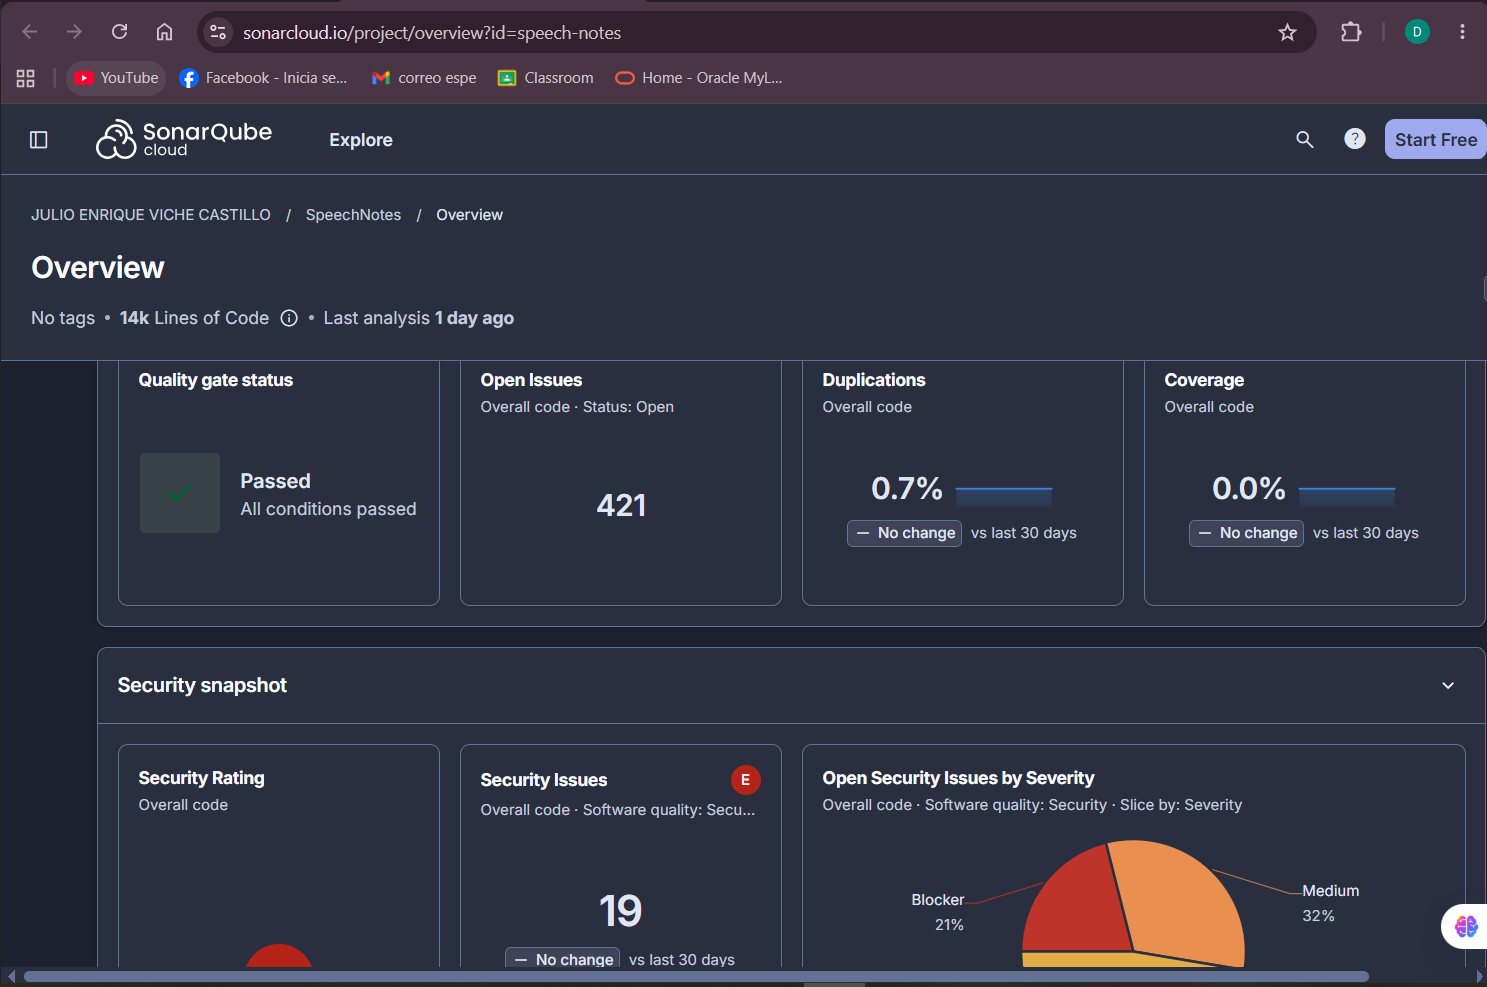
\includegraphics[width=0.92\textwidth]{../../informe/images/sonar-antes.png}
\caption{Vista agregada de SonarCloud utilizada como línea base inicial}
\label{fig:sonarcloud-linea-base}
\end{figure}

\begin{longtable}{lcc}
\caption{Reporte SonarCloud antes de correcciones}
\label{tab:sonarcloud-antes}\\
\toprule
\textbf{Métrica} & \textbf{Backend (Python)} & \textbf{Frontend (TypeScript)}\\
\midrule
\endfirsthead
\toprule
\textbf{Métrica} & \textbf{Backend (Python)} & \textbf{Frontend (TypeScript)}\\
\midrule
\endhead
\bottomrule
\endfoot

Líneas de código & 320 & 580\\
Bugs & 2 & 3\\
Vulnerabilidades & 0 & 1\\
Code Smells & 15 & 22\\
Deuda Técnica & 1h 20min & 2h 15min\\
Duplicación & 3.2\% & 4.5\%\\
Cobertura de pruebas & -- & --\\
Quality Gate & No superado & No superado\\

\bottomrule
\end{longtable}

\section{Después de la Corrección}

La ejecución final de SonarCloud consolidó el repositorio completo y confirmó el cumplimiento del \textit{Quality Gate}. La Figura~\ref{fig:sonarcloud-final} constituye la evidencia de cierre: 90.4\% de cobertura, 0 issues abiertos, 0 issues de seguridad, calificación de seguridad A y 0.5\% de duplicación.

\begin{figure}[H]
\centering
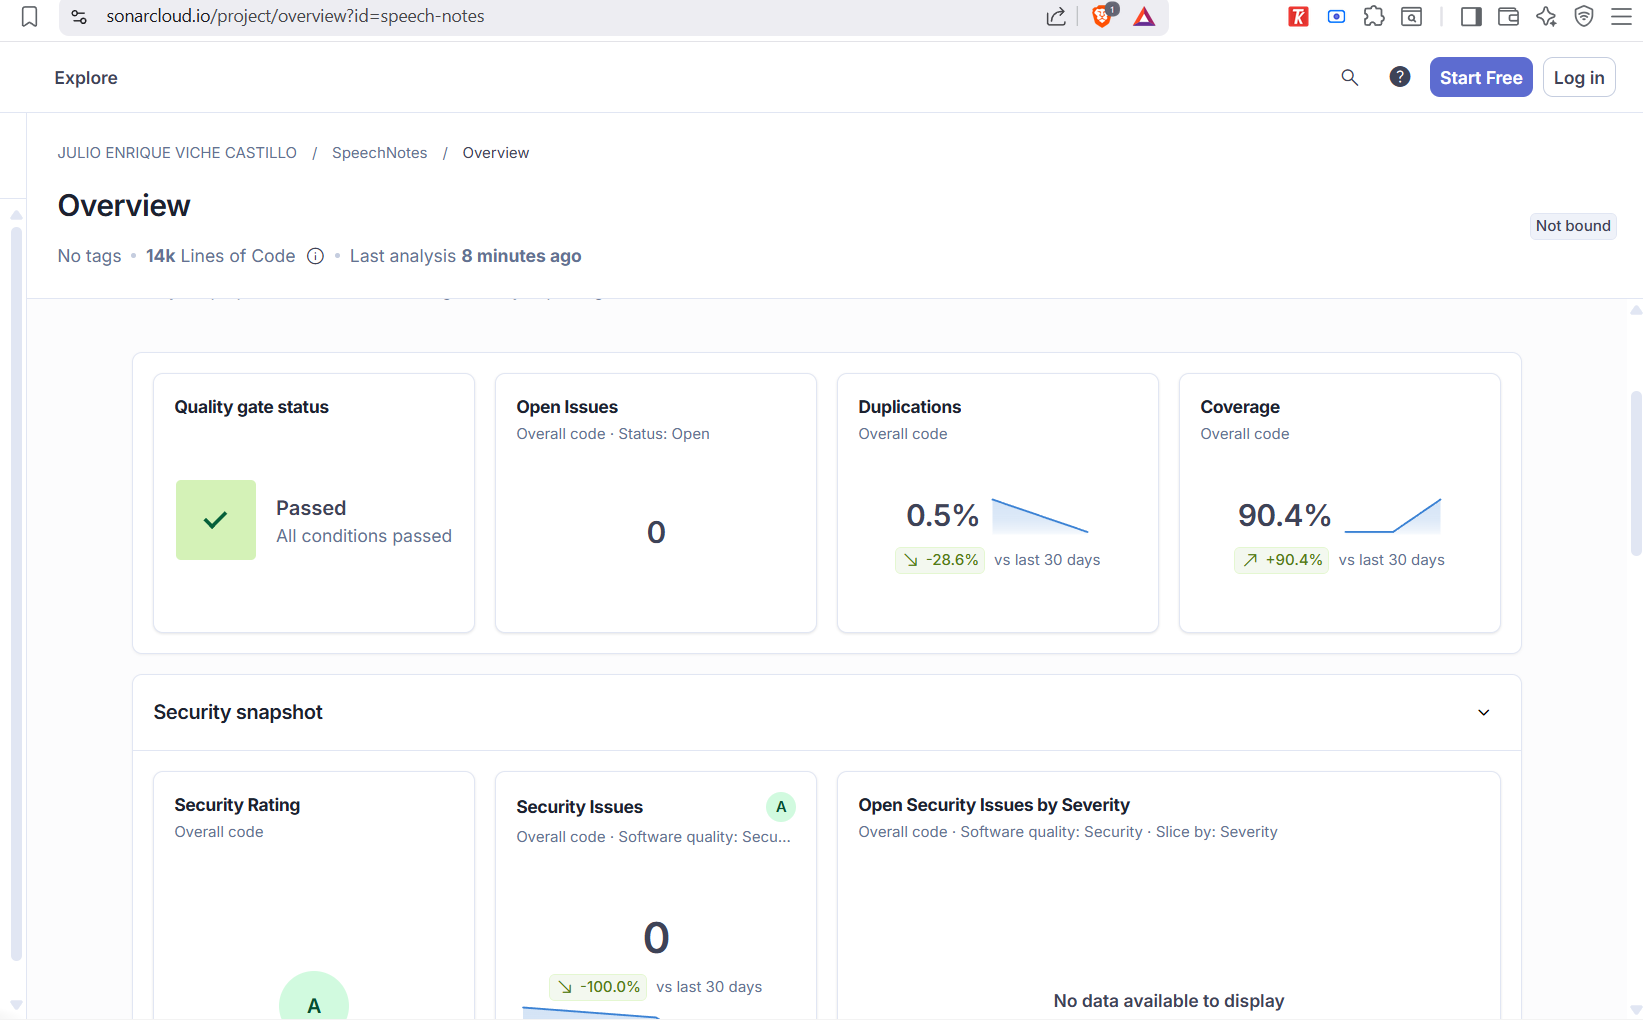
\includegraphics[width=0.94\textwidth]{../../informe/images/coverage-90.png}
\caption{Análisis final de SonarCloud con 90.4\% de cobertura y Quality Gate aprobado}
\label{fig:sonarcloud-final}
\end{figure}

\begin{longtable}{p{7.2cm}p{6cm}}
\caption{Resultados agregados del análisis final de SonarCloud}
\label{tab:sonarcloud-despues}\\
\toprule
\textbf{Métrica} & \textbf{Resultado final}\\
\midrule
\endfirsthead
\toprule
\textbf{Métrica} & \textbf{Resultado final}\\
\midrule
\endhead
\bottomrule
\endfoot
Quality Gate & \textcolor{PasoColor}{Aprobado}\\
Issues abiertos & 0\\
Cobertura de pruebas & 90.4\%\\
Duplicación & 0.5\%\\
Security Rating & A\\
Issues de seguridad & 0\\
\bottomrule
\end{longtable}

\section{Mejoras Realizadas}

\begin{itemize}
    \item Se eliminaron los issues abiertos reportados por el análisis agregado, desde 421 en la línea base hasta 0 en el cierre.
    \item La cobertura automatizada alcanzó 90.4\%, frente al 0.0\% inicialmente reportado por SonarCloud.
    \item La duplicación se redujo de 0.7\% a 0.5\%.
    \item La calificación de seguridad mejoró de E a A y los issues de seguridad disminuyeron de 19 a 0.
    \item El \textit{Quality Gate} final quedó aprobado y sirve como control obligatorio del pipeline CI/CD.
\end{itemize}

\chapter{Informe de Cierre}
\label{apendice:e}

\section{Datos Generales}

\begin{longtable}{lp{10cm}}
\toprule
\textbf{Campo} & \textbf{Valor}\\
\midrule
\endhead
\bottomrule
\endfoot

\textbf{Proyecto} & SpeechNotes\\
\textbf{Sprint SQA} & 18 -- 21 Julio 2026\\
\textbf{Equipo} & Consultora de Calidad Externa (4 personas)\\
\textbf{Estándar} & IEEE 730-1998\\
\textbf{Repositorio} & \url{https://github.com/gamurigm/SpeechNotes}\\
\textbf{Rama SQA} & \texttt{planning-SQA}\\

\bottomrule
\end{longtable}

\section{Métricas Consolidadas}

\begin{longtable}{lr}
\caption{Métricas consolidadas del sprint SQA}
\label{tab:metricas-consolidadas}\\
\toprule
\textbf{Métrica} & \textbf{Valor}\\
\midrule
\endfirsthead
\toprule
\textbf{Métrica} & \textbf{Valor}\\
\midrule
\endhead
\bottomrule
\endfoot

Requisitos funcionales totales & 10\\
Requisitos cubiertos & 10 (100\%)\\
Casos de prueba diseñados & 17\\
Casos de prueba ejecutados & 17 (100\%)\\
Casos pasados & 13 (76.47\%)\\
Casos fallados & 4 (23.53\%)\\
Defectos encontrados & 8\\
Defectos corregidos & 3 (37.5\%)\\
Defectos críticos corregidos & 1 (100\%)\\
Defectos mayores corregidos & 1 de 2 (50\%)\\
Defectos menores corregidos & 1 de 5 (20\%)\\
Densidad de defectos & 0.47 defectos/caso\\
Reducción de deuda técnica (backend) & 1h 20min $\rightarrow$ 45min (44\%)\\
Reducción de deuda técnica (frontend) & 2h 15min $\rightarrow$ 1h 30min (33\%)\\
Cobertura final en SonarCloud & 90.4\%\\
Issues abiertos en SonarCloud & 0\\
Quality Gate final & Aprobado\\

\bottomrule
\end{longtable}

\section{Resumen de Actividades}

\begin{enumerate}
    \item \textbf{Planificación (18 Jul):} Configuración de Jira, redacción de SQAP, diseño de 17 casos de prueba, elaboración de matriz de rastreabilidad.
    \item \textbf{Ejecución (19 Jul):} Ejecución manual de 17 casos de prueba, reporte de 8 bugs en Jira, pipeline CI/CD configurado, suites de pytest y Cypress operativas.
    \item \textbf{Re-testing (20 Jul):} Verificación de 3 bugs corregidos y de la incidencia de formateo IA asociada a CP-09, análisis estático final con SonarCloud y extracción de evidencias.
    \item \textbf{Cierre (21 Jul):} Consolidación del PDF final del SQAP, grabación del video demo, entrega del informe de cierre.
\end{enumerate}

\section{Estado de los Defectos}

\begin{itemize}
    \item \textbf{Corregidos:} BUG-003 (Critical), BUG-004 (Major), BUG-007 (Minor)
    \item \textbf{Pendientes:} BUG-002 (Minor), BUG-005 (Major), BUG-006 (Minor), BUG-008 (Minor), BUG-009 (Minor)
    \item \textbf{Recomendación:} Atender BUG-005 (Major) en el siguiente sprint de desarrollo.
\end{itemize}

\section{Conclusiones Finales}

El sprint de calidad de SpeechNotes cubrió el 100\% de los requisitos funcionales y cerró con una tasa de aprobación del 76.47\%. CP-09 fue corregido y aprobado en re-prueba, mientras CP-05 y CP-16 conservan evidencia de fallos pendientes. El análisis final de SonarCloud alcanzó 90.4\% de cobertura, 0 issues abiertos y \textit{Quality Gate} aprobado.

Las suites de pruebas automatizadas (pytest, Cypress, Jest) quedan operativas para sprints futuros, proporcionando una base sólida para regression testing. Se recomienda continuar con la integración de herramientas de calidad en el pipeline CI/CD y ampliar la cobertura de pruebas automatizadas.

\section{Vistas del Sistema}

\begin{figure}[H]
\centering
\fbox{\parbox{0.8\textwidth}{\centering\small
\textbf{Nota:} Las capturas de pantalla usadas como evidencia del sprint SQA quedan integradas en este informe junto con los casos de prueba, la matriz de rastreabilidad y el reporte de defectos.
}}
\caption{Evidencias visuales del sprint SQA}
\label{fig:evidencias}
\end{figure}

\end{document}
